\newif\ifTechRep
\TechRepfalse

\pdfminorversion=7
\documentclass[sigconf]{acmart}
\usepackage[font=small, labelformat=simple]{subcaption}
\usepackage[font=small, labelformat=simple]{caption}
\usepackage[ruled,vlined,noend]{algorithm2e}
\usepackage{enumitem}
\usepackage{color}
\usepackage{multicol}
\usepackage{multirow}
\usepackage{array}
\usepackage{color, colortbl}
\usepackage{booktabs}
\usepackage{balance}
\usepackage{rotating}
\usepackage{pdfrender}
\usepackage{stmaryrd}
\usepackage{anyfontsize}
\usepackage{amsthm}
\usepackage{soul}
\usepackage{xcolor}
\usepackage{soul}

\setlist{nolistsep,leftmargin=*}
\definecolor{vlightgray}{gray}{0.85}
\pdfsuppresswarningpagegroup=1
\let\paragraph\relax 

%\theoremstyle{lemma}
\newtheorem{theorem}{Theorem}
\newtheorem{definition}[theorem]{Definition}
\newtheorem{proposition}[theorem]{Proposition}
\newtheorem{lemma}[theorem]{Lemma}
\newtheorem{example}[theorem]{Example}

\newcommand{\invariant}{constraint\xspace}
\newcommand{\invariants}{constraints\xspace}
\newcommand{\Invariant}{Constraint\xspace}
\newcommand{\Invariants}{Constraints\xspace}
\newcommand{\DI}{Conformance Constraint\xspace}
\newcommand{\DIs}{Conformance Constraints\xspace}
\newcommand{\di}{conformance constraint\xspace}
\newcommand{\dis}{conformance constraints\xspace}
\newcommand{\Di}{Conformance constraint\xspace}
\newcommand{\Dis}{Conformance constraints\xspace}
\newcommand{\hdi}{conformance-constraint\xspace}

\renewcommand{\thesubtable}{(\alph{subtable})}
\renewcommand{\thesubfigure}{(\alph{subfigure})}
\newcommand{\paragraph}[1]{\noindent\textbf{#1}}
\newcommand{\affmark}[1]{\textsuperscript{\small \textsuperscript{\small #1}}}
\newcommand{\affilmark}[1]{\textsuperscript{\small #1}}
\newcommand{\ignore}[1]{{}}
\newcommand{\revise}[1]{{\color{blue} #1}}
\newcommand{\system}{\textsc{CCSynth}\xspace}
\newcommand{\nc}{unsafe\xspace}
\newcommand{\Nc}{Unsafe\xspace}
\newcommand{\extune}{SysX\xspace}
\newcommand{\View}{Projection\xspace}
\newcommand{\Views}{Projections\xspace}
\newcommand{\view}{projection\xspace}
\newcommand{\views}{projections\xspace}
\newcommand{\maxand}{\rhd}
\newcommand{\norm}{\mathtt{simp}}

\newcommand{\techRepCitation}{\ifTechRep  (see Appendix)\xspace\else \cite{technicalReport}\xspace\fi}
\newcommand{\citeTechRep}{\cite{technicalReport}}
\newcommand{\theTechRep}{our technical report~\citeTechRep}
\newcommand{\appOrTechRep}{\ifTechRep the Appendix\xspace\else our technical report~\citeTechRep\xspace\fi}

\newcommand{\af}[1]{[\textcolor{magenta}{Anna: #1}]}
\newcommand{\am}[1]{[\textcolor{magenta}{Alexandra: #1}]}
\newcommand{\at}[1]{[\textcolor{magenta}{Ashish: #1}]}
\newcommand{\mathcolorbox}[2]{\colorbox{#1}{$\displaystyle #2$}}


% Changes specific to reviewers are color coded
\definecolor{green}{RGB}{0,140,0}

% \newcommand{\green}{green}
% \newcommand{\blue}{blue}
% \newcommand{\red}{red}

%% Uncomment during camera-ready
\newcommand{\green}{black}
\newcommand{\blue}{black}
\newcommand{\red}{black}

\newcommand{\reviseone}[1]{{\color{\green} #1}}
\newcommand{\revisetwo}[1]{{\color{\blue} #1}}
\newcommand{\revisethree}[1]{{\color{\red} #1}}


\AtBeginDocument{%
  \providecommand\BibTeX{{%
    \normalfont B\kern-0.5em{\scshape i\kern-0.25em b}\kern-0.8em\TeX}}}

% Copyright

\copyrightyear{2021}
\acmYear{2021}
\setcopyright{acmlicensed}
\acmConference[SIGMOD '21] {Proceedings of the 2021 International Conference on Management of Data}{June 20--25, 2021}{Virtual Event, China}
\acmBooktitle{Proceedings of the 2021 International Conference on Management of Data (SIGMOD '21), June 20--25, 2021, Virtual Event, China}
\acmPrice{15.00}
\acmDOI{10.1145/3448016.3452795}
\acmISBN{978-1-4503-8343-1/21/06}




% remove copyright block for submission
%\setcopyright{none}
\settopmatter{printacmref=true}
%\renewcommand\footnotetextcopyrightpermission[1]{} 
%\pagestyle{plain}
\fancyhead{}
\begin{document}

\title[]{Conformance Constraint Discovery: \\Measuring Trust in Data-Driven Systems}
\ifTechRep
\subtitle{Technical Report}
\fi


\author{Anna Fariha}
\authornote{Part of the research was done while the author was an intern at Microsoft.}
\authornote{Both authors contributed equally to this research.}
\affiliation{
  \institution{University of Massachusetts Amherst}
    \institution{}
  \country{}
}
\email{afariha@cs.umass.edu}

\author{Ashish Tiwari}
\authornotemark[2]
\author{Arjun Radhakrishna}
\author{Sumit Gulwani}
\affiliation{
  \institution{Microsoft}
  \country{}
}
\email{{astiwar, arradha, sumitg}@microsoft.com}

\author{Alexandra Meliou}
\affiliation{
  \institution{University of Massachusetts Amherst}
    \institution{}
	\country{}
}
\email{ameli@cs.umass.edu}

\renewcommand{\shortauthors}{Fariha and Tiwari, et al.}
\begin{abstract}
%!TEX root = paper.tex
%
\looseness-1 The reliability of inferences made by data-driven systems hinges
on the data's continued conformance to the systems' initial settings and
assumptions. When serving data (on which we want to apply inference) deviates
from the profile of the initial training data, the outcome of inference becomes
unreliable. 
%
We introduce \emph{conformance constraints}, a new data profiling primitive
tailored towards quantifying the degree of \emph{non-conformance}, which can
effectively characterize if inference over that tuple is \emph{untrustworthy}.
%
\Dis are constraints over certain
arithmetic expressions (called \emph{projections}) involving the numerical
attributes of a dataset, which existing data profiling primitives such as
functional dependencies and denial constraints cannot model.
%
Our key finding is that projections that incur \emph{low variance} on a dataset
construct effective \dis. This principle yields the surprising result that
low-variance components of a principal component analysis, which are usually
discarded for dimensionality reduction, generate stronger \dis than the
high-variance components. Based on this result, we provide a highly scalable
and efficient technique---linear in data size and cubic in the number of
attributes---for discovering conformance constraints for a dataset. To measure
the degree of a tuple's non-conformance with respect to a dataset, we propose a
\emph{quantitative semantics} that captures how much a tuple violates the \dis
of that dataset.
%
We demonstrate the value of \dis on two applications: \emph{trusted machine
learning} and \emph{data drift}. We empirically show that \dis offer mechanisms
to (1)~reliably detect tuples on which the inference of a machine-learned model
should not be trusted, and (2)~quantify data drift more accurately than the
state of the art.
\end{abstract}

\maketitle
\fancyhead{}

\section{Introduction}\label{sec:introduction}
%!TEX root = paper.tex

\looseness-1 
%Data is central to modern systems in a wide range of domains.
%, including healthcare, transportation, and finance. 
The core of modern data-driven systems typically comprises of models learned
from large datasets, and they are usually optimized to target particular data
and workloads. While these data-driven systems have seen wide adoption and
success, their reliability and proper functioning hinge on the data's continued
conformance to the systems' initial settings and assumptions. When the serving
data (on which the system operates) deviates from the profile of the initial
data (on which the system was trained), system performance degrades and system
behavior becomes unreliable. Therefore, a mechanism to assess the
trustworthiness of a system's inferences is paramount, especially for systems
that perform safety-critical or high-impact operations.

A machine-learned (ML) model typically works best if the serving dataset
follows the profile of the dataset the model was trained on; when it doesn't,
the model's inference can be unreliable. One can profile a dataset in many
ways, such as by modeling the data distribution of the
dataset~\cite{achlioptas2017learning}, or by finding the (implicit)
\emph{constraints} that the dataset satisfies~\cite{pena2019discovery}.
Distribution-oriented approaches learn data likelihood (e.g., joint or
conditional distribution) from the training data, and can be used to check if
the serving data is unlikely. An unlikely tuple does not necessarily imply that
the model would fail for it. The problem with the distribution-oriented
approaches is that they tend to overfit, and, thus, are overly conservative
towards unseen tuples, leading them to report many such false positives.

\looseness-1 We argue that certain constraints offer a more effective and
robust mechanism to quantify trust of a model's inference on a serving tuple.
The reason is that learning systems implicitly exploit such constraints during
model training, and build models that assume that the constraints will continue
to hold for serving data. For example, when there exist high correlations among
attributes in the training data, learning systems will likely reduce the
weights assigned to redundant attributes that can be deduced from others, or
eliminate them altogether through dimensionality reduction. If the serving data
preserves the same correlations, such operations are inconsequential;
otherwise, we may observe model failure.

\looseness-1 In this paper, we characterize datasets with a new data-profiling
primitive, \emph{\dis}, and we present a mechanism to identify \emph{strong}
\dis, whose violation indicates unreliable inference. \Dis specify constraints
over \emph{arithmetic relationships} involving multiple numerical attributes of
a dataset. We argue that a tuple's conformance to the \dis is more critical for
accurate inference than its conformance to the training data distribution. This
is because any violation of \dis is likely to result in a catastrophic failure
of a learned model that is built upon the assumption that the \dis will always
hold. Thus, we can use a tuple's deviation from the \dis as a proxy for the
trust on a learned model's inference for that tuple. We proceed to describe a
real-world example of \dis, drawn from our case-study evaluation on
\emph{trusted machine learning} (TML).

\setlength{\tabcolsep}{.5em}
\renewcommand{\arraystretch}{.9}
\begin{figure}[t]
\centering
    \resizebox{1\columnwidth}{!}
	{\small
	
    \begin{tabular}{lcccc}
    \toprule
     							& \textbf{Departure} 		& \textbf{Departure Time} 		& \textbf{Arrival Time} 		& \textbf{Duration (min)} 	\\
								& \textbf{Date} 	 		& \textbf{[DT]} 				&  \textbf{[AT]} 				& \textbf{[DUR]} 		  	\\
    \midrule
		$t_1$ 					& May 2 					& \texttt{14:30} 				& \texttt{18:20}  				& 230 					  	\\
		$t_2$ 					& July 22 					& \texttt{09:05}				& \texttt{12:15}  				& 195 					  	\\
        \revisetwo{$t_3$} 		& 	\revisetwo{June 6} 		& \revisetwo{\texttt{10:20}}	  & \revisetwo{\texttt{12:20}}  & \revisetwo{115} 			\\ 
		$t_4$ 					& May 19 					& \texttt{11:10} 				& \texttt{13:05}  			   	& 117 						\\
		\rowcolor{vlightgray}
		$t_5$ 					& April 7 					& \texttt{22:30}  			  & \texttt{06:10}  			  	& 458						\\

    \bottomrule
    \end{tabular}
    }
	\vspace{-3mm}
    \caption{\small
	%
	 Sample of the airlines dataset (details are in
	 Section~\ref{exp-invariants-for-ML}), showing departure, arrival, and
	 duration only. The dataset does not report arrival date, but an arrival time
	 earlier than departure time (e.g., last row), indicates an overnight flight.
	 \reviseone{All times are in 24 hour format} and in the same time zone. There is some
	 noise in the values.
	%
	} 
	\vspace{-2mm}
    \label{fig:flights}
\end{figure}

\begin{example}\label{ex:tml}
	\looseness-1

We used a dataset with flight information that includes data on departure and
arrival times, flight duration, etc.\ (Fig.~\ref{fig:flights}) to train a
linear regression model to predict flight delays. \revisetwo{The model was
trained on a subset of the data that happened to include only daytime flights
(such as the first four tuples)}. In an empirical evaluation of the regression
accuracy, we found that the mean absolute error of the regression output more
than quadruples for overnight flights (such as the last tuple $t_5$), compared
to daytime flights. The reason is that tuples representing overnight flights
deviate from the profile of the training data \revisetwo{that only contained
daytime flights}. Specifically, daytime flights satisfy the \di that ``arrival
time is later than departure time and their difference is very close to the
flight duration'', which does not hold for overnight flights. Note that this
\invariant is just based on the covariates (predictors) and does not involve
the target attribute $\mathtt{delay}$. Critically, although this \di is unaware
of the regression task, it was still a good proxy of the regressor's
performance. \revisetwo{In contrast, approaches that model data likelihood may
report long daytime flights as unlikely, since all flights in the training data
($t_1$--$t_4$) were also short flights, resulting in false alarms, as the model
works very well for most daytime flights, regardless of the duration (i.e., for
both short and long daytime flights).}
	%
\end{example}

\revisetwo{Example~\ref{ex:tml} demonstrates that when training data has
\emph{coincidental} relationships (e.g., the one between $\mathtt{AT}$,
$\mathtt{DT}$, and $\mathtt{DUR}$ for daytime flights), then ML models may
\emph{implicitly} assume them as \emph{invariants}. \Dis can capture such data
invariants and flag non-conforming tuples (overnight flights) during
serving.}\label{extake}

\smallskip

\paragraph{\Dis.} \Dis complement the existing data profiling literature, as
the existing constraint models, such as functional dependencies and denial
constraints, cannot model arithmetic relationships. For example, the \di of
Example~\ref{ex:tml} is: $-\epsilon_1 \le \mathtt{AT} - \mathtt{DT} -
\mathtt{DUR} \le \epsilon_2$, where $\epsilon_1$ and $\epsilon_2$ are small
values. \Dis can capture complex linear dependencies across attributes within a
\emph{noisy} dataset. For example, if the flight departure and arrival data
reported the hours and the minutes across separate attributes, the \invariant
would be on a different arithmetic expression: $(60\cdot \mathtt{arrHour} +
\mathtt{arrMin}) - (60\cdot \mathtt{depHour} + \mathtt{depMin}) -
\mathtt{duration}$.

\looseness-1 The core component of a \di is the arithmetic expression, called
\emph{projection}, which is obtained by a linear combination of the numerical
attributes. There is an unbounded number of projections that we can use to form
arbitrary \dis. For example, for the projection $\mathtt{AT}$, we can find a
broad range $[\epsilon_3, \epsilon_4]$, such that all training tuples in
Example~\ref{ex:tml} satisfy the \di $\epsilon_3 \le \mathtt{AT} \le
\epsilon_4$. However, this \invariant is too inclusive and a learned model is
unlikely to exploit such a weak constraint. In contrast, the projection
$\mathtt{AT} - \mathtt{DT} - \mathtt{DUR}\;$ leads to a stronger \di with a
narrow range as its bounds, which is selectively permissible, and, thus, more
effective.

\smallskip

\paragraph{Challenges and solution sketch.} The principal challenge is to
discover an \emph{effective} set of conformance constraints that are likely to
affect a model's inference implicitly. We first characterize ``good''
projections (that construct effective constraints) and then propose a method to
discover them. We establish through theoretical analysis two important results:
(1)~A projection is good over a dataset if it is almost constant (i.e., has low
variance) over all tuples in that dataset. (2)~A set of projections,
collectively, is good if the projections have small pair-wise correlations. We
show that low variance components of a principal component analysis (PCA) on a
dataset yield such a set of \views. Note that this is different from---and, in
fact, completely opposite of---the traditional approaches
(e.g.,~\cite{DBLP:conf/kdd/QahtanAWZ15}) that perform multidimensional analysis
based on the high-variance principal components, after reducing dimensionality
using PCA.

\smallskip

\paragraph{Scope.} \looseness-1 Fig.~\ref{relatedWorkMatrix} summarizes prior
work on related problems, but our scope differs significantly. Specifically, we
can detect if a serving tuple is non-conforming with respect to the training
dataset \emph{only based on its predictor attributes}, and require no knowledge
of the ground truth. This setting is essential in many practical applications
when we observe \emph{extreme verification latency}~\cite{souzaSDM:2015}, where
ground truths for serving tuples are not immediately available. For example,
consider a self-driving car that is using a trained controller to generate
actions based on readings of velocity, relative positions of obstacles, and
their velocities. In this case, we need to determine, only based on the sensor
readings (predictors), when the driver should be alerted to take over vehicle
control.
%, as we cannot use ground-truths to generate an alert.
%
Furthermore, we \emph{do not assume access to the model}, i.e., model's
predictions on a given tuple. This setting is necessary for (1)~safety-critical
applications, where the goal is to quickly alert the user, without waiting for
the availability of the prediction, (2)~auditing and privacy-preserving
applications where the prediction cannot be shared, and (3)~when we are unaware
of the detailed functionality of the system due to privacy concerns or lack of
jurisdiction.
% , but only have some
% meta-information such as the system trains some linear model over the training
% data.
%
We focus on identifying \emph{tuple-level} non-conformance as opposed to
dataset-level non-conformance that usually requires observing entire data's
distribution. However, our tuple-level approach trivially extends (by
aggregation) to the entire dataset.

%!TEX root = paper.tex

\newcolumntype{?}{!{\vrule width 1pt}}
\newcommand{\sln}{2}
\newcommand{\eln}{18} 
\newcommand{\cm}{\checkmark}
\newcommand{\gm}{!}
\let\st\relax
\newcommand{\st}{$\star$}
\newcommand{\na}{$\bot$}
\newcommand{\nr}{$\varoslash$}
\newcommand*{\bc}{% bold checkmark
  \textpdfrender{
    TextRenderingMode=FillStroke,
    LineWidth=.5pt,
  }{\checkmark}
}

\begin{figure}[t] 
	\setlength\tabcolsep{1pt} 
	\centering	
	%\renewcommand{\arraystretch}{1.0}
	\resizebox{1\columnwidth}{!}{ \small 
	\begin{tabular}
		{?c|c|p{50mm}?c|c|c|c|c|c?p{3mm}|c?c|c|c?c|c|c|c?c|c?} 
		
		\hline
		
		\hline
		
		\multicolumn{3}{?c?}{\cellcolor{vlightgray}{\multirow[c]{1}{*}{\cellcolor{vlightgray}{\rotatebox[origin=lb]{0}{{\textbf{Legend}}}}}}} & 
		
		% High-level Aspects
		\multicolumn{6}{c?}{{\multirow[c]{1}{*}{\rotatebox[origin=lb]{0}{{\scriptsize constraints}}} }} &
		\multicolumn{2}{c?}{{\multirow[c]{1}{*}{\rotatebox[origin=lb]{0}{{\scriptsize violation}}}}} &
		\multicolumn{3}{c?}{{\multirow[c]{1}{*}{\rotatebox[origin=lb]{0}{{\scriptsize setting}}}}} &
		\multicolumn{4}{c?}{{\multirow[c]{1}{*}{\rotatebox[origin=lb]{0}{{\scriptsize technique}}}}} &
		\multicolumn{2}{c?}{{\multirow[c]{1}{*}{\rotatebox[origin=lb]{0}{{\scriptsize TML}}}}}\\
		\hline
		
		\hline

		% Legends
		\multicolumn{2}{?r}{\cellcolor{vlightgray}{\small HP:	}} & 			\multicolumn{1}{l?}{\cellcolor{vlightgray}\small Hyper Parameter } &&&&&&&&&&&&&&&&&\\
		\multicolumn{2}{?r}{\cellcolor{vlightgray}{\small FD:	}} & 			\multicolumn{1}{l?}{\cellcolor{vlightgray}\small Functional Dependency} &&&&&&&&&&&&&&&&&\\
		\multicolumn{2}{?r}{\cellcolor{vlightgray}{\small DC:	}} & 			\multicolumn{1}{l?}{\cellcolor{vlightgray}\small Denial Constraint}		&&&&&&&&&&&&&&&&&\\
		\multicolumn{2}{?r}{\cellcolor{vlightgray}{\small \nr:	}} & 			\multicolumn{1}{l?}{\cellcolor{vlightgray}\small Does not require } &&&&&&&&&&&&&&&&&\\
		\multicolumn{2}{?r}{\cellcolor{vlightgray}{\small \na:	}} & 			\multicolumn{1}{l?}{\cellcolor{vlightgray}\small Not applicable } &&&&&&&&&&&&&&&&&\\
		\multicolumn{2}{?r}{\cellcolor{vlightgray}{\small \st:	}} & 			\multicolumn{1}{l?}{\cellcolor{vlightgray}\small Supports via extension} &&&&&&&&&&&&&&&&&\\
		\multicolumn{2}{?r}{\cellcolor{vlightgray}{\small !:	}} & 			\multicolumn{1}{l?}{\cellcolor{vlightgray}\small Partially}& 		 
		
		% Constraints aspects	 
		\multirow[t]{4}{*}{\begin{sideways}{{\small parametric}}\end{sideways}} &
		\multirow[t]{4}{*}{\begin{sideways}{{\small arithmetic}}\end{sideways}} &
		\multirow[t]{4}{*}{\begin{sideways}{{\small approximate}}\end{sideways}} &	
		\multirow[t]{4}{*}{\begin{sideways}{{\small conditional}}\end{sideways}}&
		\multirow[t]{4}{*}{\begin{sideways}{{\small notion of weight}}\end{sideways}} &
		\multirow[t]{4}{*}{\begin{sideways}{{\small interpretable}}\end{sideways}} &

		% Violation aspects
		\multirow[t]{4}{*}{\begin{sideways}{{\small continuous}}\end{sideways}} &
		\multirow[t]{4}{*}{\begin{sideways}{{\small tuple-wise}}\end{sideways}} &

		% Setting aspects
		\multirow[t]{4}{*}{\begin{sideways}{{\small noisy data}}\end{sideways}} &
		\multirow[t]{4}{*}{\begin{sideways}{{\small numerical attr.}}\end{sideways}} &
		\multirow[t]{4}{*}{\begin{sideways}{{\small categorial attr.}}\end{sideways}} &
		
		% Technique aspects
		\multirow[t]{4}{*}{\begin{sideways}{{\small $\!\varoslash\!$ thresholds}}\end{sideways}} &
		\multirow[t]{4}{*}{\begin{sideways}{{\small $\!\varoslash\!$ distance metric}}\end{sideways}} &
		\multirow[t]{4}{*}{\begin{sideways}{{\small $\!\varoslash\!$ HP tuning}}\end{sideways}}&
		\multirow[t]{4}{*}{\begin{sideways}{{\small scalable}}\end{sideways}} &

		% TML aspects
		\multirow[t]{4}{*}{\begin{sideways}{{\small task agnostic}}\end{sideways}} &
		\multirow[t]{4}{*}{\begin{sideways}{{\small $\!\varoslash\!$ access to model}}\end{sideways}}\\
		
		\hline 
		
		\hline
		
		% Data Profiling techniques
		\multirow{13}{*}{\begin{sideways}{Data Profiling}\end{sideways}} & 
		 
						   \multicolumn{2}{l?}{\textbf{\DIs} } 																&\bc&\bc&\bc&\bc&\bc&\st&	\multicolumn{1}{c|}{\bc} &\bc&	\bc&\bc	&\bc&		\bc&\bc &\bc&\bc&		\bc&\bc\\
		\cline{\sln-20}& \multicolumn{2}{l?}{FD~\cite{papenbrock2015functional}} 											&	&	&	&	&	&\cm&		&	&	   &	&\cm&	\cm&\cm &\cm&   &		\multicolumn{2}{c?}{\multirow{12}{*}{\begin{sideways}{not addressed in prior work}\end{sideways}}}\\
		\cline{\sln-\eln}& \multicolumn{2}{l?}{Approximate FD~\cite{kruse2018efficient}} 									&	&	&\cm&	&	&\cm&		&	&	\cm&	&\cm&	   &\cm &\cm&	&	  \multicolumn{2}{c?}{}\\
		\cline{\sln-\eln}& \multicolumn{2}{l?}{Metric FD~\cite{koudas2009metric}} 											&	&	&\cm&	&	&\cm&		&	&	\cm&\cm	&\cm&	   &	&\na&\na&	  \multicolumn{2}{c?}{}\\
		\cline{\sln-\eln}& \multicolumn{2}{l?}{Conditional FD~\cite{DBLP:conf/icde/FanGLX09}} 								& ! &	&	&\cm&	&\cm&		&\cm&	\cm&	&\cm&	   &\cm &\cm&   &	  \multicolumn{2}{c?}{}\\
		\cline{\sln-\eln}& \multicolumn{2}{l?}{Pattern FD~\cite{qahtan2020pattern}} 										& ! &	&	&	&	&\cm&		&\cm&	\cm&	&\cm&	   &\cm &\cm&   &	  \multicolumn{2}{c?}{}\\		
		\cline{\sln-\eln}& \multicolumn{2}{l?}{Soft FD~\cite{DBLP:conf/sigmod/IlyasMHBA04}} 								&	&	&\cm&	&\cm&\cm&	\cm &	&	\cm&\cm	&\cm&	   &\cm &\cm&\cm&	  \multicolumn{2}{c?}{}\\
		\cline{\sln-\eln}& \multicolumn{2}{l?}{Relaxed FD~\cite{caruccio2016discovery}} 									&	&	&\cm&	&	&\cm&		&	&	\cm&\cm	&\cm&	   &	&\cm&	&	  \multicolumn{2}{c?}{}\\
		\cline{\sln-\eln}& \multicolumn{2}{l?}{FDX~\cite{DBLP:conf/sigmod/ZhangGR20}} 										&	&	&	&	&	&\cm&		&	&	\cm&	&\cm&	   &	&	&\cm&	  \multicolumn{2}{c?}{}\\
		\cline{\sln-\eln}& \multicolumn{2}{l?}{Differential Dependency~\cite{song2011differential}} 						&	&	&	&	&	&\cm&		&	&	   &\cm	&\cm&	   &	&\cm&	&	  \multicolumn{2}{c?}{}\\
		\cline{\sln-\eln}& \multicolumn{2}{l?}{DC~\cite{DBLP:journals/pvldb/ChuIP13, DBLP:journals/pvldb/BleifussKN17}} 	& ! &	&\cm&\cm&\cm&\cm&		&\cm&	\cm&\cm	&\cm&	   &\cm &\cm&	&	  \multicolumn{2}{c?}{}\\
		\cline{\sln-\eln}& \multicolumn{2}{l?}{Approximate DC~\cite{pena2019discovery, DBLP:journals/corr/abs-2005-08540}} 	& ! &	&\cm&\cm&\cm&\cm&		&\cm&	\cm&\cm	&\cm&	   &\cm &\cm&	&	  \multicolumn{2}{c?}{}\\
		\cline{\sln-\eln}& \multicolumn{2}{l?}{Statistical Constraint~\cite{DBLP:conf/sigmod/YanSZWC20}} 					&	&	&\cm&	&	&\cm&	\cm	&	&	\cm&\cm &\cm&	   &\cm &\cm&\cm&	  \multicolumn{2}{c?}{}\\
			
		\hline
						
		\hline
		
		% Learning Techniques	
		\multirow{7}{*}{\begin{sideways}{Learning}\end{sideways}} & 
						   \multicolumn{2}{l?}{Ordinary Least Square} 														&\cm&\cm&\cm&	&	&\st		&\cm&\cm		&\cm&\cm&\st		&\cm&\cm&\cm&\cm		&	&	\\
		\cline{\sln-20}& \multicolumn{2}{l?}{Total Least Square} 															&\cm&\cm&\cm&	&	&\st		&\cm&\cm		&\cm&\cm&\st		&\cm&\cm&\cm&\cm		&\cm&\cm\\
		\cline{\sln-20}& \multicolumn{2}{l?}{Auto-encoder~\cite{DBLP:journals/corr/abs-1812-02765}} 						&\multicolumn{6}{c?}{\na}		&\cm&\cm		&\cm&\cm&\cm		&	&	&	&\cm		&\cm&\cm\\
		\cline{\sln-20}& \multicolumn{2}{l?}{Schelter et al.~\cite{DBLP:conf/sigmod/SchelterRB20}\textsuperscript{+}} 	&\multicolumn{6}{c?}{\na}		&\cm&			&	&\cm&\cm		&	&\cm&\cm&\cm		&	&	\\
		\cline{\sln-20}& \multicolumn{2}{l?}{Jiang et al.~\cite{DBLP:conf/nips/JiangKGG18}} 								&\multicolumn{6}{c?}{\na}		&\cm&\cm		&\cm&\cm&\cm		&\cm&	&	&\cm		&	&	\\
		\cline{\sln-20}& \multicolumn{2}{l?}{Hendrycks et al.~\cite{DBLP:journals/corr/HendrycksG16c}} 					&\multicolumn{6}{c?}{\na}		&	&\cm		&\cm&\cm&\cm		&\cm&\cm&\cm&\cm		&	&	\\
		\cline{\sln-20}& \multicolumn{2}{l?}{Model's Prediction Probability} 												&\multicolumn{6}{c?}{\na}		&\cm&\cm		&\multicolumn{7}{c?}{varies}				&   &	\\
		\hline
		
		\hline
		\multicolumn{20}{r}{\textsuperscript{+} {\scriptsize Requires additional information}}\\

	\end{tabular}
	} 	
	\vspace{-4mm} 	
	\caption{\Dis complement existing data profiling primitives and provide an 
	efficient mechanism to quantify trust in prediction, with
	minimal assumption on the setting. 
    } 
	\label{relatedWorkMatrix} 
	\vspace{-4mm} 
	
\end{figure}


\smallskip

\paragraph{Contrast with prior art.} We now discuss where \dis fit with respect
to the existing literature (Fig.~\ref{relatedWorkMatrix}).
% on data profiling and literature on modeling trust in data-driven inferences 

\looseness-1 \subsubsection*{Data profiling techniques} \Dis fall under the
umbrella of data profiling, which refers to the task of extracting~tech\-nical
metadata about a given dataset~\cite{DBLP:journals/vldb/AbedjanGN15}. A key
task in data profiling is to learn relationships among attributes. Functional
dependencies (FD)~\cite{papenbrock2015functional} and their variants only
capture if a relationship exists between two sets of attributes, but do not
provide a closed-form (parametric) expression of the relationship. Using the FD
``$\{\mathtt{AT}, \mathtt{DT}\} \rightarrow$ $\{\mathtt{DUR}\}$'' to model the
\invariant of Example~\ref{ex:tml} suffers from several limitations. First,
since the data is noisy, no exact FD can be learned. Metric
FDs~\cite{koudas2009metric} allow small variations in the data,
% (similar
% attribute values are considered identical), 
but hinge on appropriate distance metrics and thresholds. For example, if
$\mathtt{time}$ is split across two attributes ($\mathtt{hour}$ and
$\mathtt{minute}$), the distance metric is non-trivial: it needs to encode that
$\langle \mathtt{hour} = 4, \mathtt{min} = 59 \rangle$ and $\langle
\mathtt{hour} = 5, \mathtt{min} = 1\rangle$ are similar, while $\langle
\mathtt{hour} = 4, \mathtt{min} = 1\rangle$ and $\langle \mathtt{hour} = 5,
\mathtt{min} = 59\rangle$ are not. In contrast, \dis can model the composite
attribute ($60 \cdot \mathtt{hour} + \mathtt{minute}$) by automatically
discovering the coefficients $60$ and $1$.
% for such a composite attribute.

\looseness-1 Denial constraints (DC)~\cite{DBLP:journals/pvldb/ChuIP13,
DBLP:journals/pvldb/BleifussKN17, pena2019discovery,
DBLP:journals/corr/abs-2005-08540} encapsulate a number of different
data-profiling primitives such as FDs and their variants (e.g,~\cite{
DBLP:conf/icde/FanGLX09}). Exact DCs can adjust to noisy data by adding
predicates until the constraint becomes exact over the entire dataset, but this
can make the constraint extremely large and complex, which might even fail to
provide the desired generalization. For example, a finite DC---whose language
is limited to universally quantified first-order logic---cannot model the
constraint of Example~\ref{ex:tml}, which involves an arithmetic expression
(addition and multiplication with a constant). Expressing \dis requires a
richer language that includes linear arithmetic expressions. \revisetwo{Pattern
functional dependencies (PFD)~\cite{qahtan2020pattern} move towards addressing
this limitation of DCs, but they focus on text attributes: they are regex-based
and treat digits as characters. However, modeling arithmetic relationships of
numerical attributes requires interpreting digits as numbers.}

\looseness-1 To adjust for noise, FDs and DCs either relax the notion of
constraint violation or allow a user-defined fraction of tuples to violate the
(strict) constraint~\cite{pena2019discovery, huhtala1999tane,
kruse2018efficient, DBLP:conf/sigmod/IlyasMHBA04, koudas2009metric,
caruccio2016discovery, DBLP:journals/corr/abs-2005-08540}. Some
approaches~\cite{DBLP:conf/sigmod/IlyasMHBA04, DBLP:conf/sigmod/ZhangGR20,
DBLP:conf/sigmod/YanSZWC20} use statistical techniques to model other types of
data profiles such as correlations and conditional dependencies. However, they
require additional parameters such as noise and violation thresholds and
distance metrics. In contrast, \dis do not require any parameter from the user
and work on noisy datasets.

\revisetwo{Existing data profiling techniques are not designed to learn what ML
models exploit and are sensitive to noise in the numerical attributes.
Moreover, data constraint discovery algorithms typically search over an
exponential set of candidates, and hence, are not scalable: their complexity
grows exponentially with the number of attributes or quadratically with data
size. In contrast, our technique for deriving \dis is highly scalable (linear
in data size) and efficient (cubic in the number of attributes). It does not
explicitly explore the candidate space, as PCA---which lies at the core of our
technique---performs the search \emph{implicitly} by iteratively refining
weaker \invariants to stronger ones.} \label{nocandidate}

\subsubsection*{Learning techniques} While \emph{ordinary least square} finds
the lowest-variance projection, it minimizes observational error on only the
target attribute, and, thus, does not apply to our setting. \emph{Total least
square} offers a partial solution as it takes observational errors on all
predictor attributes into account; but, it finds only one projection---the
lowest variance one---that fits the data tuples best. But there may exist other
projections with slightly higher variances and we consider them all. As we show
empirically in Section~\ref{exp-invariants-for-drift}, constraints derived from
multiple projections, collectively, capture various aspects of the data, and
result in an effective data profile targeted towards certain tasks such as
data-drift quantification~\citeTechRep.

\medskip 

\paragraph{Contributions.} We make the following contributions:

\begin{itemize}

     \item We ground the motivation of our work with two case studies on trusted
     machine learning (TML) and data drift. (Section~\ref{sec:casestudies})
     
     \item We introduce and formalize \dis, a new data profiling primitive that
     specifies constraints over arithmetic relationships among numerical
     attributes of a dataset. We describe a \emph{conformance language} to
     express \dis, and a \emph{quantitative semantics} to quantify how much a
     tuple violates the \dis. In applications of constraint violations, some
     violations may be more or less critical than others. To capture that, we
     consider a notion of \invariant importance, and weigh violations against
     \invariants accordingly. (Section~\ref{sec:data-invs})
      
     \item We formally establish that strong \dis are constructed from
     projections with small variance and small mutual correlation on the given
     dataset. Beyond simple linear \invariants (e.g., the one in
     Example~\ref{ex:tml}), we derive \emph{disjunctive} \invariants, which are
     disjunctions of linear \invariants. We achieve this by dividing the
     dataset into disjoint partitions, and learning linear \invariants for each
     partition. We provide an efficient, scalable, and highly parallelizable
     algorithm for computing a set of linear \dis and disjunctions over them.
     We also analyze its runtime and memory complexity.
     (Section~\ref{sec:synth-data-inv})
     
     \item We formalize the notion of \emph{\nc} tuples in the context of
     trusted machine learning and provide a mechanism to detect \nc tuples
     using \dis. (Section~\ref{sec:di-for-tml})
	 
     \item We empirically analyze the effectiveness of \dis in two case-study
     applications---TML and data-drift quantification. We show that \dis can
     reliably predict the trustworthiness of linear models and quantify data
     drift precisely, outperforming the state of the art.
     (Section~\ref{sec:experiments})
	 
  \end{itemize}

\section{Case Studies}\label{sec:casestudies}
%!TEX root = paper.tex
% \section{Case Studies}

\looseness-1 Like other data-profiling primitives, \dis have general
applicability in understanding and describing datasets. However, their true
power lies in quantifying the degree of a tuple's non-conformance with respect
to a reference dataset. Within the scope of this paper, we focus on two case
studies
%in particular 
to motivate our work.
%: trusted machine learning and data drift. 
We provide an extensive evaluation over these applications in
Section~\ref{sec:experiments}.

% , which can be used to determine whether the prediction of a
% learned model can be trusted on a new serving
% tuple.Furthermore, . 

\smallskip

\looseness-1 \paragraph{Trusted machine learning (TML)} refers to the problem
of quantifying trust in the inference made by a machine-learned model on a new
serving tuple~~\cite{DBLP:conf/hicons/TiwariDJCLRSS14,
DBLP:journals/crossroads/Varshney19, DBLP:journals/corr/abs-1904-07204,
DBLP:conf/kdd/Ribeiro0G16, DBLP:conf/nips/JiangKGG18}.
%
\ignore{
This is particularly useful in
case of extreme verification latency~\cite{souzaSDM:2015}, where ground-truth
outputs for new serving tuples are not immediately available to evaluate the
performance of a learned model, when auditing models for trustworthiness, and
in privacy-preserving applications where even the model's predictions cannot be
shared.
}
%
When a model is trained using a dataset, the \dis for that dataset specify a
safety envelope~\cite{DBLP:conf/hicons/TiwariDJCLRSS14} that characterizes the
tuples for which the model is expected to make trustworthy predictions. If a
serving tuple falls outside the safety envelope (violates the \dis), then the
model is likely to produce an untrustworthy inference. Intuitively, the higher
the violation, the lower the trust. Some classifiers produce a confidence
measure along with the class prediction, typically by applying a softmax
function to the raw numeric prediction values. However, such confidence
measures are not well-calibrated~\cite{DBLP:conf/nips/JiangKGG18,
guo2017calibration}, and, therefore, cannot be reliably used as a measure of
trust in the prediction. Additionally, a similar mechanism is not available for
inferences made by regression models.

\looseness-1 In the context of TML, we formalize the notion of \emph{\nc
tuples}, on which the prediction may be untrustworthy. We establish that \dis
provide a sound and complete procedure for detecting \nc tuples, which
indicates that the search for \dis should be guided by the class of models
considered by the corresponding learning system (Section~\ref{sec:di-for-tml}).

% Since our
% proof of this result is non-constructive, we present a second result that
% establishes sufficient, but not necessary, conditions for solving it
% . 


\smallskip

\paragraph{Data drift}~\cite{DBLP:conf/kdd/QahtanAWZ15,
DBLP:journals/tnn/KunchevaF14, DBLP:journals/csur/GamaZBPB14,
DBLP:journals/jss/BarddalGEP17} specifies a significant change in a dataset
with respect to a reference dataset, which typically requires that systems be
updated and models retrained.
% Aggregating tuple-level non-conformances over a
% dataset gives us a \emph{dataset-level} non-conformance, which is an effective
% measurement of data drift.
To quantify how much a dataset $D'$ drifted from a reference dataset $D$, our
three-step approach is: (1)~compute \dis for $D$, (2)~evaluate the \invariants
on all tuples in $D'$ and compute their violations (degrees of
non-conformance), and (3)~finally, aggregate the tuple-level violations to get
a dataset-level violation. If all tuples in $D'$ satisfy the \invariants, then
we have no evidence of drift. Otherwise, the aggregated violation serves as the
drift quantity.

\smallskip

While we focus on these two applications here, we mention other applications of
\dis in \appOrTechRep.








\section{\DIs}\label{sec:data-invs}
%!TEX root = paper.tex
%% \section{\DIs}

\def\Inv{\mathtt{Inv}}
\def\Dom{\mathtt{Dom}}
\def\coDom{\mathtt{coDom}}
\def\DDom{\mathbf{Dom}}
\def\CC{\mathcal{C}}
\def\Real{{\mathbb{R}}}
%\def\dist{{\mathtt{qmem}}}

\def\Bool{{\mathtt{Bool}}}
\def\true{{\mathtt{True}}}
\def\false{{\mathtt{False}}}
\def\vecw{{\vec{w}}}
\def\vecv{{\vec{v}}}
\def\lb{{\mathtt{lb}}}
\def\ub{{\mathtt{ub}}}
\def\atomic{{atomic}}
\def\Atomic{{Atomic}}
%\def\M{{\infty}}
%\def\Conj{{\varphi}}
%\def\Disj{{\Phi}}
\newcommand{\semq}[1]{{[\![{#1}]\!]}}
%\newcommand\avg[1]{{\overline{#1}}}
\newcommand\avg[1]{{\mathtt{\mu}}(#1)}
\newcommand\sign[1]{{\mathtt{sign}({#1})}}
\newcommand\delF[2]{{\Delta{#1}({#2})}}
\newcommand\stddev[1]{{\mathtt{\sigma}}(#1)}
\def\monthy{M}


In this section, 
%we define \dis that allow us to capture complex arithmetic dependencies involving numerical attributes of a dataset. 
we first provide the general definition of \dis. Then we propose a language for
representing them. Finally, we define quantitative semantics over \dis, which
allows us to quantify their violation.

% We present one possible \emph{language} for representing \dis,
% and attach a \emph{quantitative semantics} to it.
% The quantitative semantics, intuitively, computes the degree of
% \invariant violation on data.
%Finally, we provide a principle for synthesizing effective \dis. 
% Finally, we discuss how we prioritize
% \invariants during quantitative semantics computation based on their
%effectiveness.

\smallskip
% \noindent \textbf{tuple, attribute, and Dataset.}

\looseness-1
\paragraph{Basic notation.}
%
We use $\mathcal{R} (A_1, A_2, \dots, A_m)$ to denote a relation schema where
$A_i$ denotes the $i^{th}$ attribute of $\mathcal{R}$. We use $\Dom_i$ to
denote the domain of attribute $A_i$. Then the set ${\DDom}^m=\Dom_1\times
\cdots\times \Dom_m$ specifies the domain of all possible tuples. We use $t
\in\DDom^m$ to denote a tuple in the schema $\mathcal{R}$. A dataset
$D\subseteq {\DDom}^m$ is a specific instance of the schema $\mathcal{R}$. For
ease of notation, we assume some order of tuples in $D$ and we use $t_i \in D$
to refer to the $i^{th}$ tuple and $t_i.A_j \in \Dom_j$ to denote the value of
the $j^{th}$ attribute of $t_i$.

\ignore{
\paragraph{Tuple, Dataset, and Attribute.} Let $\Dom_1, \Dom_2, \ldots, \Dom_n$
denote some $n$ domains for values. We fix the set $\Dom_1\times \cdots\times
\Dom_n$ (written as ${\DDom}^m$) as the domain of all {\em{tuples}}. Each
\emph{tuple} $d\in\DDom^m$ is an $n$-tuple, where each component of the tuple
is an {\em{attribute}}.\footnote{\scriptsize{In this work, we use the term
``attribute'' to denote a single attribute.}} We use $A_1,\ldots,x_n$ to denote
the names of these $n$ attributes. We use $d_{x_j}\in \Dom_j$ to denote the
value of the $j^{th}$ attribute of $d$. A {\em{dataset}} $D\subseteq {\DDom}^m$
is a sequence of tuples, where the $i^{th}$ tuple is denoted using $d^{(i)}$.
\endignore
}

%We differentiate between two types of attributes in a dataset, namely
%categorical and numerical. An attribute with domain $\Dom_i$ is categorical if
%$\Dom_i$ is a finite discrete set with small (e.g., up to 50) cardinality. The
%domain of a numerical attribute is the set of numbers. 

% \sloppy
% \begin{definition}[\Di]\label{def:di}
%      %
%      A \di for a dataset $D \,{\subseteq}\, {\DDom}^m$ is another
%      dataset $\Inv \,{\subseteq}\, {\DDom}^m$ s.t. $D - {D'} \,{\subseteq}\,
%      \Inv$, and $\frac{|D'|}{|D|} \le \delta$.
%      %
% \end{definition}

\ignore{
\smallskip
\looseness-1 We start with a \emph{strict} definition of \dis, and then explain how it generalizes to account for noise in the data.
% 
\begin{definition}[\Di (strict)]\label{def:di}
     %
     A \di for a dataset $D \,{\subseteq}\, {\DDom}^m$ is a formula $\Phi:
     \DDom^m \mapsto \{\true,\false\}$ such that $\forall t\in D,
     \Phi(t) = \true$.
     %
\end{definition}
% 

\looseness-1
A \di ($\Phi$) characterizes a set of allowable or conforming tuples and is
expressed through a \emph{conformance language} (Section~\ref{sec:cl}). We write
$\Phi(t)$ and $\neg\Phi(t)$ to denote that $t$ satisfies and violates the
\invariant $\Phi$, respectively. In practice, because of noise, some tuples in
$D$ may violate a \invariant. To account for noise, we relax the definition of
\di as follows.
\endignore}
% %
% \looseness-1 We start with a formal definition of \dis, which is a formula
% expressed in a \emph{conformance language} (Section~\ref{sec:cl}),
% that is satisfied by almost all tuples in $D$.

\smallskip
% \noindent \textbf{tuple, attribute, and Dataset.}

\looseness-1 \paragraph{\Di.} A \di $\Phi$ characterizes a set of allowable or
conforming tuples and is expressed through a \emph{conformance language}
(Section~\ref{sec:cl}). We write $\Phi(t)$ and $\neg\Phi(t)$ to denote that $t$
satisfies and violates $\Phi$, respectively.

\begin{definition}[\Di]\label{def:di2}
     %
     A \di for a dataset $D \,{\subseteq}\, {\DDom}^m$ is a formula
     $\Phi: {\DDom}^m \mapsto \{\true,\false\}$ such that $|\{t \in D \mid
     \neg\Phi(t)\}| \ll |D|$.
	 %
\end{definition}
% 
The set $\{t \in D \mid \neg\Phi(t)\}$ denotes atypical tuples in $D$ that do
not satisfy the \di $\Phi$. In our work, we do not need to know the set of
atypical tuples, nor do we need to purge the atypical tuples from the dataset.
Our techniques derive \invariants in ways that ensure there are very few
atypical tuples (Section~\ref{sec:synth-data-inv}). 


\subsection{Conformance Language}\label{sec:cl}
%
\looseness-1 \paragraph{\View.} A central concept in our conformance language
is \linebreak \emph{\view}. Intuitively, a \view is a derived attribute that
specifies a ``lens'' through which we look at the tuples. More formally, a
\view is a function $F: \DDom^m \mapsto\Real$ that maps a tuple $t\in\DDom^m$
to a real number $F(t) \in \Real$. In our language for \dis, we only consider
\views that correspond to linear combinations of the numerical attributes of a
dataset. Specifically, to define a \view, we need a set of numerical
coefficients for all attributes of the dataset and the \view is defined as a
sum over the attributes, weighted by their corresponding coefficients. We extend
a projection $F$ to a dataset $D$ by defining $F(D)$ to be the sequence of
reals obtained by applying $F$ on each tuple in $D$ individually.

\smallskip

{
%\setlength{\abovedisplayskip}{0pt}
%\setlength{\belowdisplayskip}{0pt}
\paragraph{Grammar.} Our language for \dis consists of formulas
$\Phi$ generated by the following grammar:
%
{
\begin{eqnarray*}
    \phi & := & \lb \leq F(\vec{A}) \leq \ub \; \mid\; \wedge(\phi,\ldots,\phi)
    \\[-0.3em]
    \psi_A & := & \vee(\;(A = c_1) \maxand \phi,\; (A = c_2) \maxand \phi, \;\ldots)
    \\[-0.3em]
    \Psi & := & \psi_A \; \mid \; \wedge(\psi_{A_1}, \psi_{A_2}, \ldots)
	\\[-0.3em]
    \Phi & := & \phi  \;\mid\; \Psi
\end{eqnarray*}
}
%
% The language consists of
% (1)~equality constraints $A_j = c_j$ where $A_j$ is an attribute and $c_j \in \Dom_j$ is a concrete value;
% (2)~bounded \view constraints $\lb \leq F(\vec{A}) \leq \ub$ where
%     $F$ is a \view on $\DDom^m$, $\vec{A}$ is the tuple of formal
%     parameters $(A_1, A_2, \ldots, A_m)$, and $\lb, \ub \in \Real$ are reals; and
% (3)~their conjunctions ($\wedge$) and disjunctions ($\vee$).
%   %
  %
\looseness-1 
\noindent 
The language consists of (1)~bounded constraints $\lb \leq F(\vec{A})\leq \ub$
where $F$ is a \view on $\DDom^m$, $\vec{A}$ is the tuple of formal parameters
$(A_1, A_2, \ldots, A_m)$, and $\lb, \ub \in \Real$ are reals; (2)~equality
constraints $A = c$ where $A$ is an attribute and $c$ is a constant in
$A$'s domain; and (3)~operators ($\maxand$, $\wedge$, and $\vee$,) that connect
the constraints.
}
%where the first two are intuitively conjunctive and  and $\wedge$ are two conjunction operators and $\vee$ is a disjunctions ($\vee$).
  % conjunction $\wedge$ and disjunction $\vee$ operators are variable arity operators.
Intuitively, $\maxand$ is a switch operator that specifies which \invariant $\phi$
applies based on the value of the attribute $A$, $\wedge$ denotes conjunction,
and $\vee$ denotes disjunction.
% $\vee$ and $\wedge$ are the usual Boolean operators. We allow an
% equality $x = c$ to be part of a \di only when $x$ is categorical.
Formulas generated by $\phi$ and $\Psi$ are called {\em{simple \invariants}}
and {\em{compound \invariants}}, respectively. Note that a formula generated by
$\psi_A$ only allows equality constraints on a single attribute, namely $A$,
among all the disjuncts.
% Then $\Psi$ generates a
% \emph{compound \invariant} which is a conjunction over a set of disjunctive
% \invariants (on different attributes). Finally, $\Phi$ gives either a
% conjunctive \invariant or a compound \invariant.

\begin{example}\label{ex:constraints}
    Consider the dataset $D$ consisting of the first four tuples  $\{t_1, t_2, t_3, t_4\}$ of Fig.~\ref{fig:flights}.
    A simple \invariant for $D$ is:
	{
	$$
    \phi_1: -5\leq \mathtt{AT} - \mathtt{DT} - \mathtt{DUR} \leq 5.
	$$
	}
	%
    Here, the projection ${F(\vec{A})} = \mathtt{AT} - \mathtt{DT} - \mathtt{DUR}$, with attribute coefficients
    $\langle 1, - 1, -1 \rangle$, $\lb = {-}5$, and $\ub = 5$. A compound
    \invariant is:
	%
	{
	\begin{align*}
     \psi_2:   \mathtt{\monthy} &= \text{``May''}  \maxand -2 \leq \mathcolorbox{lightgray}{\mathtt{AT} - \mathtt{DT} - \mathtt{DUR}} \leq 0 \\[-0.4em]
     \vee \;\; \mathtt{\monthy} &= \text{``June''} \maxand \phantom{-}0  \leq \mathcolorbox{lightgray}{\mathtt{AT} - \mathtt{DT} - \mathtt{DUR}} \leq 5\\[-0.4em]
     \vee \;\; \mathtt{\monthy} &= \text{``July''} \, \maxand {-}5 \leq \mathcolorbox{lightgray}{\mathtt{AT} - \mathtt{DT} - \mathtt{DUR}} \leq 0
	\end{align*}
	}
	 %
     For ease of exposition, we assume that all times are converted to minutes
     (e.g., \texttt{06:10} $= 6 \times 60 + 10 = 370$) and $\monthy$ denotes
     the departure month, extracted from $Departure$ $Date$.
	 %
\end{example}

Note that arithmetic expressions that specify linear combination of numerical
attributes (highlighted above) are disallowed in denial
constraints~\cite{DBLP:journals/pvldb/ChuIP13} which only allow raw attributes
and constants (more details are in \appOrTechRep).




\subsection{Quantitative Semantics}\label{quant-sem}

\looseness-1 \Dis have a natural Boolean semantics: a tuple either satisfies a
\invariant or it does not. However, Boolean semantics is of limited use in
practice, because it does not quantify the degree of \invariant violation. We
interpret \dis using a quantitative semantics, which quantifies violations, and
% to handle noisy data.
% This is important because data can be noisy and
%Quantitative semantics has the additional benefit that it 
reacts to noise more gracefully than Boolean semantics.

%Given a formula $\Phi$,
% and a tuple $d$,
The quantitative semantics $\semq{\Phi}(t)$ is a measure of the violation of
$\Phi$ on a tuple $t$---with a value of $0$ indicating no violation and a value
greater than 0 indicating some violation. In Boolean semantics, if $\Phi(t)$ is
$\true$, then $\semq{\Phi}(t)$ will be $0$; and if $\Phi(t)$ is $\false$, then
$\semq{\Phi}(t)$ will be $1$. Formally, $\semq{\Phi}$ is a mapping from
$\DDom^m$ to $[0,1]$.

\smallskip

\noindent\emph{Quantitative semantics of simple \invariants.} 
%
\revisethree{We build upon $\epsilon$-insen\-sitive loss~\cite{vapnik1997support}
to define the quantitative semantics of simple \invariants, where the bounds
$\lb$ and $\ub$ define the $\epsilon$-insensitive
zone:}\footnote{\revisethree{For a target value $y$, predicted value $\hat{y}$,
and a parameter $\epsilon$, the $\epsilon$-insensitive loss is $0$ if $|y -
\hat{y}| < \epsilon$ and $|y - \hat{y}| - \epsilon$ otherwise.
% $\epsilon$-insensitive loss is defined by $
% %
%         \begin{cases}
%         0, & \text{if } |y - \hat{y}| < \epsilon\\
%         |y - \hat{y}| - \epsilon, & \text{otherwise}
%         \end{cases}
%   $
}}\label{fn1}
%
\begin{align*}
    \semq{\lb\leq F(\vec{A})\leq \ub}(t) &:= \eta(\alpha \cdot \max(0, F(t)-\ub, \lb - F(t)))
    \\
    \semq{\wedge(\phi_1,\ldots,\phi_K)}(t) &:= \textstyle\sum_{k}^{K} \gamma_k \cdot \semq{\phi_k}(t)
\end{align*}
%
Below, we describe the parameters of the quantitative semantics, and provide further details on them in \appOrTechRep.
% The quantitative semantics uses the following parameters:\footnote{More details on system parameters are in \appOrTechRep.}
% \begin{itemize}
%   \item a \emph{scaling factor} $\alpha\in\Real^+$,
%   \item a \emph{normalization function} $\eta(.): \Real\mapsto [0,1]$, and
%   \item \emph{importance factors} $\gamma_k \in \Real^+$ s.t. $\sum \gamma_k = 1$.
% \end{itemize}
% %and $\gamma_i$'s---which are non-negative real numbers whose sum is $1$---denote \emph{importance factors}.
% We discuss these parameters next.

\smallskip 
% \sloppy \noindent \textbf{Scaling factor $\alpha$.}
\paragraph{Scaling factor $\alpha\in\Real^+$.}\\ \Views are unconstrained
functions and different \views can map the same tuple to vastly different
values. We use a scaling factor $\alpha$ to standardize the values computed by
a \view $F$, and to bring the values of different \views to the same comparable
scale. The scaling factor is automatically computed as the inverse of the
standard deviation, $\alpha = \tfrac{1}{\stddev{F(D)}}$. 
We set $\alpha$ to a large positive number when $\stddev{F(D)}$ = $0$.

% A typical choice---inspired from the classical z-score normalization---is the inverse of standard deviation
% of $F(D)$, i.e., $1/\stddev{F(D)}$.\footnote{\scriptsize{When $\stddev{F(D)}$ = $0$, we use a large positive number $\M$ as the scaling factor.}}

\smallskip
% \sloppy \noindent \textbf{Normalization function $\eta$.}
\paragraph{Normalization function $\eta(.): \Real\mapsto [0,1]$.}\\
The normalization function
maps values in the range $[0,\infty)$ to the range $[0,1)$.
While any monotone mapping from $\Real^{\geq 0}$ to $[0,1)$ can be used, we
pick $\eta(z) = 1 - e^{-z}$.

\smallskip 
% \noindent\textbf{Importance factors $\gamma_i$.} 
\looseness-1
\paragraph{Importance factors $\gamma_k\in \Real^+$, $\textstyle\sum_{k}^{K}\gamma_k {=} 1$.}\\
The weights $\gamma_k$ control the contribution of each bounded-\view \invariant in a
conjunctive formula. This allows for prioritizing \invariants that are more
significant than others.
% within the context of a particular application.
In our work, we derive the importance factor of a \invariant automatically,
based on its \view's standard deviation over $D$.

\subsubsection*{Quantitative semantics of compound \invariants} 
Compound \invariants are first simplified into simple \invariants, and they get
their meaning from the simplified form.
We define a function
$\norm(\psi, t)$ that takes a compound \invariant $\psi$ and a tuple $t$ and returns a simple
\invariant. It is defined recursively as follows:
\begin{align*}
    &\norm(\vee(\;(A = c_1) \maxand\phi_1, (A = c_2) \maxand \phi_2,\ldots), t) := 
      \phi_k  \; \mbox{if $t.A = c_k$}
    \\
    &\norm(\wedge(\psi_{A_1}, \psi_{A_2},\ldots), t)  := \wedge(\norm(\psi_{A_1}, t), \norm(\psi_{A_2},t),\ldots)
\end{align*}
%
\begin{sloppypar} If the condition in the definition above does not hold for any $c_k$, then
$\norm(\psi,t)$ is undefined and $\norm(\wedge(\dots,\psi,\dots),t)$ is
also undefined. If $\norm(\psi,t)$ is undefined, then $\semq{\psi}(t) :=
1$. When $\norm(\psi,t)$ is defined, the quantitative semantics of $\psi$ is
given by:
$$
\semq{\psi}(t) := \semq{\norm(\psi,t)}(t)
$$
\end{sloppypar}

Since compound \invariants simplify to simple \invariants, we mostly focus on 
simple \invariants. Even there, we pay special attention to bounded-projection 
\invariants ($\phi$) of the form \linebreak $\lb \le F(\vec{A}) \le \ub$, which lie at the core of simple \invariants. 


\begin{example}\label{ex:semantics}
	%
    Consider the \invariant $\phi_1$ from Example~\ref{ex:constraints}.
	%
    % denoting $-5\leq F(\vec{A}) \leq 5$, where $F(\vec{A}) = AT - DT -
%     DUR$, over the database $D$ consisting of the first four tuples,
%     $\{t_1, t_2, t_3, t_4\}$, shown in Fig.~\ref{fig:flights}.
	%
	For $t \in D$,
    $\semq{\phi_1}(t)= 0$ since $\phi_1$ is satisfied by all tuples in $D$. The
    standard deviation of the projection $F$ over $D$, $\sigma(F(D)) {=}
    \sigma(\{0,-5, 5, -2\}) {=} 3.6$. Now consider the last tuple $t_5 \not\in
    D$. $F(t_5) = (370 - 1350)-458 = -1438$, which is way below the lower bound $-5$ of $\phi_1$. 
	Now we compute how much $t_5$ violates $\phi_1$: 
	$\semq{\phi_1}(t_5) = \semq{-5 \leq F(\vec{A}) \leq 5}(t_5) 
		 			   = \eta(\alpha \cdot \max(0, -1438 - 5, -5 + 1438)) = 1 - e^{-\frac{1433}{3.6}} \approx 1$.
%		 			   &= 1 - e^{-\frac{1433}{\sigma(F(D))}} = 1 - e^{-\frac{1433}{3.6}} \approx 1
%	\end{align*}
	%
	Intuitively, this implies that $t_5$ strongly violates $\phi_1$.
	%
\end{example}




\section{\DI Synthesis}\label{sec:synth-data-inv}
%!TEX root = paper.tex
% \section{Synthesizing \DIs}

\looseness-1 In this section, we describe our techniques for deriving \dis. We
start with the synthesis of simple \invariants (the $\phi$ \invariants in
our language specification), followed by compound \invariants (the $\Psi$
\invariants in our language specification). Finally, we analyze the time and
memory complexity of our algorithm.

\subsection{Simple \DIs}\label{sec:conjunctive} Synthesizing simple \dis
involves (a)~discovering the \views, and (b)~discovering the lower and upper
bounds for each \view. We start by discussing~(b), followed by the principle to
identify effective \views, based on which we solve~(a).


\subsubsection{Synthesizing Bounds for \Views}\label{synth-bounds} Fix a \view $F$
and consider the bounded-\view \invariant $\phi$: $\lb \leq
F(\vec{A}) \leq \ub$. 
% Now, the tightest bounds for this form, for a dataset $D$,
% is given by $\ub = \max(F(D))$ and $\lb = \min(F(D))$.
% However, this choice is very sensitive to noise:
% adding a single ``atypical'' tuple to $D$ can produce very different
% \invariants.
Given a dataset $D$, a trivial choice for the bounds
% valid on all tuples in a dataset $D$ 
is: $\lb = \min(F(D))$ and $\ub = \max(F(D))$. However, this choice is very
sensitive to noise: adding a single atypical tuple to $D$ can produce very
different \invariants.
% To concretize the \invariant, we need to instantiate
% the \view $F$, and the bounds $\lb$ and $\ub$.
% We provide a constructive
% mechanism to synthesize \views for linear \invariants in
% Section~\ref{sec:pca-invs}. Here, we focus on the constants $\lb$ and $\ub$.
% For a \view $F$, we compute $\lb$ and $\ub$ as follows:
%
% However, it suffers from two issues: (1)~if $F(D)$ has very low variance (e.g.,
% a constant), then the \invariant may become too tight, and (2)~if there is even
% a single atypical tuple in $D$, the bound can be too loose.
% However, it suffers from two issues: (1)~if $F(D)$ has very low variance (e.g.,
% a constant), then the \invariant may become too tight, and (2)~if there is even
% a single atypical tuple in $D$, the bound can be too loose.
Instead, we use a more robust choice as follows:
%, at the cost of potentially having a small number of tuples in $D$ that do not satisfy the \invariant:
%
\begin{align*}
    \lb = \avg{F(D)} - C \cdot \stddev{F(D)}, \;\;\;\;
    \ub = \avg{F(D)} + C \cdot \stddev{F(D)}
\end{align*}
%
\looseness-1
Here, $\avg{F(D)}$ and $\stddev{F(D)}$ denote the mean and standard deviation
of the values in $F(D)$, respectively, and $C$ is some positive constant.
With these bounds, $\semq{\phi}(t) = 0$ implies that
%\begin{enumerate*}[label=(\alph*)]
    %\item 
        $F(t)$ is within $C \times \stddev{F(D)}$ from the mean $\avg{F(D)}$. % \emph{and}
    %\item $F(t)$ is between $\min(F(D))$ and $\max(F(D))$.
%\end{enumerate*}
%
%
%
%Consequently, some 
% Since there can be tuples $t\in D$ that are more than $C$ standard
% deviations away from the mean,
% % These tuples are considered outliers, and
% $\phi$ is a \invariant for the subset of $D$ that excludes some ``outliers'';
% this is often desirable for many practical applications.
% that are more then $4$ standard
% deviations away from the mean may violate $\phi$; so, $\phi$ may not be an
% \invariant for $D$, but only for some subset of $D$ that does not contain any
% outlier. 
% However, this is often desirable for many practical applications.
%
In our experiments, we set $C = 4$, which ensures that in expectation, very few
tuples in $D$ will violate the \invariant for many distributions of the values
in $F(D)$. Specifically, if $F(D)$ follows a normal distribution, then
$99.99\%$ of the population is expected to lie within $4$ standard deviations
from mean. \reviseone{Note that we make no assumption on the original data
distribution of each attribute.}


% Since a-priori we have no knowledge of the underlying distribution of the
% values in $F(D)$, we assume that the distribution is normal and therefore, we
% use $C = 4$ in our experiments.\footnote{\scriptsize{For normal distributions,
% $99.99\%$ of the population is expected to lie within $4$ standard deviations
% from mean. Only 1 in 15787 tuples falls outside this range.}}

%Note that the choice of $\lb$ and $\ub$ is not restricted to the above and one
%can follow a different design choice for computing the bounds, guided by the
%assumption of distribution of $F(D)$ in associated application.
% the quantitative semantics of data
% \invariant is not limited to this assumption and can support assumption of any
% distribution, given a procedure to compute $\lb$ and $\ub$ is available.}
%
%
% \smallskip
%
Setting the bounds $\lb$ and $\ub$ as $C\cdot\stddev{F(D)}$-away from the mean,
and the scaling factor $\alpha$ as $\frac{1}{\stddev{F(D)}}$, guarantees the
following property for our quantitative semantics:
% As long as the scaling factor $\alpha=\frac{1}{\stddev{F(D)}}$ and
% the bounds $\lb,\ub$ are given by $\avg{F(D)}\pm C*\stddev{F(D)}$ for some $C$,
% %However, regardless of the choice of bounds $\lb$ and $\ub$,
% the quantitative semantics has the following nice property.
%
\begin{figure}
	\centering
	\resizebox{0.8\columnwidth}{!}{
	\begin{subfigure}{.18\textwidth}
	  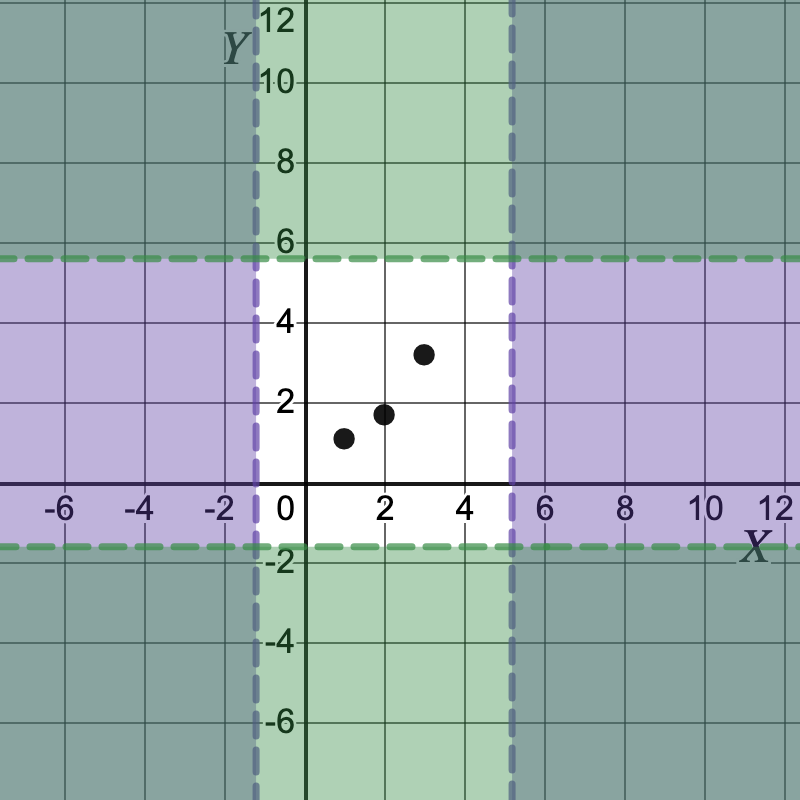
\includegraphics[width=1\linewidth]{Figures/view1.png}
	  \vspace{-6mm}
	  \caption{}
	  \label{subfig:views1}
	\end{subfigure}%
	\hspace{5mm}
	\begin{subfigure}{.18\textwidth}
	  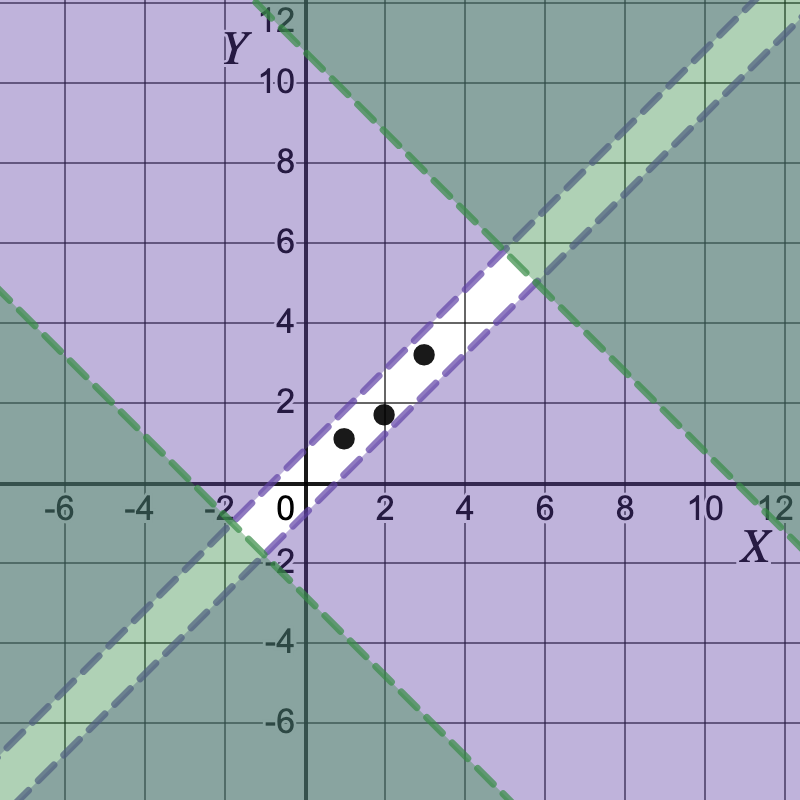
\includegraphics[width=1\linewidth]{Figures/view2.png}
	  \vspace{-6mm}
	  \caption{}
	  \label{subfig:views3}
	\end{subfigure}
	}
	\vspace{-4mm}
        \caption{\small
		\looseness-1
		Clear and shaded regions depict conformance and non-conformance zones, respectively.
		(a)~Correlated projections $X$ and $Y$ yield \dis forming a large conformance zone, % resulting in an underfitted data profile.
		(b)~Uncorrelated (orthogonal) projections $X-Y$ and $X+Y$ yield \dis forming a smaller conformance zone.%, resulting in an optimal data profile.
		}
	\label{fig:views}
	\vspace{-3mm}
\end{figure}

\begin{lemma}\label{lemma:helper}
    Let $D$ be a dataset and let 
    $\phi_k$ be $\lb_k \leq F_k(\vec{A})\leq \ub_k$ for $k=1,2$.
    Then, for any tuple $t$, if 
    $\frac{|F_1(t) - \avg{F_1(D)}|}{\stddev{F_1(D)}} \geq \frac{|F_2(t) - \avg{F_2(D)}|}{\stddev{F_2(D)}}$,
    then $\semq{\phi_1}(t) \geq \semq{\phi_2}(t)$.
\end{lemma}
%
This means that larger deviation from the mean (proportionally to
the standard deviation) results in higher degree of violation under our
semantics. The proof follows from the fact that the normalization function
$\eta(.)$ is monotonically increasing, and hence, $\semq{\phi_k}(t)$ is a
monotonically non-decreasing function of $\frac{|F_k(t) -
\avg{F_k(D)}|}{\stddev{F_k(D)}}$.


\subsubsection{Principle for Synthesizing \Views}\label{view-synthesis}
%
% \looseness-1
% One question naturally arises: what \views should we use to synthesize
% \invariants for $D$? Does it even matter what \views we pick, or would any choice
% be equally effective? To answer these questions, we need to first understand
% what makes a \invariant more effective than others for a particular task. For
% many practical applications, \invariants of \emph{moderate} strength are most
% effective. Ideally, we look for two criteria in an effective \invariant: (1)~it
% should not overfit the data, rather should generalize by capturing the
% properties of the data, (2)~it should not underfit the data, because majority
% of the tuples within the data domain would then satisfy such \invariant. To
% satisfy the first criterion, we allow flexible bounds---specified using $\lb$
% and $\ub$---as discussed earlier. To satisfy the second criterion, we
% pick \views that produce strong \invariants.
% %among a set of possible \invariants, with
% %respect to a large subset of the data domain.

\looseness-1 %To understand how to derive the \views for effective \dis, 
We start by investigating what makes a \invariant more effective than others.
An effective \invariant (1)~should not overfit the data, but rather generalize
by capturing the properties of the data, and (2)~should not underfit the data,
because it would be too permissive and fail to identify deviations effectively.
Our flexible bounds (Section~\ref{synth-bounds}) serve to avoid overfitting. In
this section, we focus on identifying the principles that help us avoid
underfitting. We first describe the key technical ideas for characterizing
effective \views through example and then proceed to formalization.

% https://www.desmos.com/calculator/zrtfddd6dn
% 
\begin{example}\label{ex:badproj}
	%
	 \looseness-1 Let $D$ be a dataset of three tuples
	 \{(1,1.1),(2,1.7),(3,3.2)\} with two attributes $X$ and $Y$. Consider two
	 arbitrary \views: $X$ and $Y$. For $X$: $\mu(X(D)) = 2$ and $\sigma(X(D)) =
	 0.8$. So, bounds for its \di are: $\lb = 2 - 4 \times 0.8 = -1.2$ and $\ub =
	 2 + 4 \times 0.8 = 5.2$. This gives us the \di: $-1.2 \le X \le 5.2$.
	 Similarly, for $Y$, we get the \di: $-1.6 \le Y \le 5.6$.
	 Fig.~\ref{subfig:views1} shows the conformance zone (clear region) defined by
	 these two \dis. The shaded region depicts non-conformance zone. The
	 conformance zone is large and too permissive: it allows many atypical tuples
	 with respect to $D$, such as $(0,4)$ and $(4, 0)$.
	%
\end{example}

A natural question arises: are there other \views that can better characterize
conformance with respect to the tuples in $D$? The answer is yes and next we
show another pair of \views that shrink the conformance zone significantly.

\begin{example}\label{ex:goodproj} 
	%
	 In Fig.~\ref{subfig:views3}, the clear region is defined by the \dis $-0.8
	 \le X - Y \le 0.8$ and $-2.8 \le X + Y \le 10.8$, over \views $X-Y$ and
	 $X+Y$, respectively. The region is indeed much smaller than the one in
	 Fig.~\ref{subfig:views1} and allows fewer atypical tuples.
	 %
\end{example}




How can we derive \view $X-Y$ from the \views $X$ and $Y$, given $D$? Note that
$X$ and $Y$ are highly correlated in $D$. In Lemma~\ref{LEMMA:MAIN}, we show
that two highly correlated \views can be linearly combined to construct another
\view with lower standard deviation that generates a \emph{stronger} \invariant.
%We later generalize this result to
%multiple \views in Theorem~\ref{THM:MAIN}. 
We proceed to formalize {\em{stronger \invariant}}---which defines whether a
\invariant is more effective than another in quantifying violation---and
\emph{incongruous tuples}---which help us estimate the subset of the data
domain for which a \invariant is stronger than the others.

\begin{definition}[Stronger \invariant]\label{def:stronger}
	\begin{sloppypar}
A \di $\phi_1$ is stronger
than another \di $\phi_2$ on a subset $H \subseteq \DDom^m$ if
$\forall t \in H, \; \semq{\phi_1}(t) \geq \semq{\phi_2}(t)$.
	\end{sloppypar}
\end{definition}

%
Given a dataset $D\subseteq \DDom^m$ and a \view $F$, for any tuple $t$, let
$\delF{F}{t} = F(t) - \avg{F(D)}$. For \views $F_1$ and $F_2$, the correlation
coefficient $\rho_{F_1,F_2}$ (over $D$) is defined as
$\frac{\frac{1}{|D|}\sum_{t\in D}
\delF{F_1}{t}\delF{F_2}{t}}{\stddev{F_1(D)}\stddev{F_2(D)}}$.
%
\begin{definition}[Incongruous tuple]	
A tuple $t$ is {\em{incongruous}} w.r.t.\ a
\view pair $\!\langle F_1, F_2\rangle\!$ on $D$ if: 
$\delF{F_1}{t}\cdot\delF{F_2}{t}\cdot\rho_{F_1,F_2}<0$.
%
\end{definition}



Informally, an incongruous tuple for a pair of \views does not follow the
general trend of correlation between the \view pair. For example, if $F_1$ and
$F_2$ are positively correlated ($\rho_{F_1,F_2}>0$), an incongruous tuple $t$
deviates in opposite ways from the mean of each \view
($\delF{F_1}{t}\cdot\delF{F_2}{t}<0$). Our goal is to find \views that yield a
conformance zone with very few incongruous tuples.

\begin{example} 
	%
	In Example~\ref{ex:badproj}, $X$ and $Y$ are positively
correlated with $\rho_{X,Y} \approx 1$. The tuple
$t=(0,4)$ is incongruous w.r.t. $\langle X, Y \rangle$, because $X(t) = 0 <
\mu(X(D)) = 2$, whereas $Y(t) = 4 > \mu(Y(D)) = 2$. Intuitively, the
incongruous tuples do not behave like the tuples in $D$ when viewed through the
\views $X$ and $Y$. Note that the narrow conformance zone of
Fig.~\ref{subfig:views3} no longer contains the incongruous tuple $(0, 4)$.
In fact, the conformance zone defined by the \dis derived from \views $X - Y$
and $X + Y$ are free from a vast majority of the incongruous tuples.
%
\end{example}


We proceed to state Lemma~\ref{LEMMA:MAIN}, which informally says that any two
highly correlated \views can be linearly combined to construct a new \view to
obtain a stronger \invariant. We write $\phi_F$ to denote the \di $\lb \le
F(\vec{A}) \le \ub$, synthesized from $F$. (All proofs are in \appOrTechRep.)



\begin{lemma}\label{LEMMA:MAIN}
    Let $D$ be a dataset and $F_1,F_2$ be two \views on $D$ s.t.\ $|\rho_{F_1,F_2}| \geq \frac{1}{2}$.
    Then, $\exists \beta_1, \beta_2 \in \Real$ s.t.\ $\beta_1^2 + \beta_2^2 = 1$ and for the new \view
    $F = \beta_1 F_1 + \beta_2 F_2$:
	 %
	 \begin{enumerate}[label=(\arabic*)]
	     \item $\stddev{F(D)} < \stddev{F_1(D)}$ and $\stddev{F(D)} < \stddev{F_2(D)}$, and
         \item $\phi_F$ is stronger than both $\phi_{F_1}$ and $\phi_{F_2}$
     on the set of tuples that are incongruous w.r.t. $\!\langle F_1,
     F_2\rangle$.
	 \end{enumerate} 
	 %
% Here $\phi_F$ just denotes $\lb \leq F(\vec{A}) \leq \ub$,
%      where $\lb,\ub$ are as defined above.
	 %
    %$\mathtt{sign}((F_1(t) - \avg{F_1(D)}) * (F_2(t) - \avg{F_2(D)}) * \rho_{F_1(D),F_2(D)}) = -1$,
\end{lemma}
%

\noindent We now extend the result to multiple \views in Theorem~\ref{THM:MAIN}.
%

\begin{theorem}[Low Standard Deviation \Invariants]\label{THM:MAIN}
	%\sloppy
    Given a dataset $D$, let $\mathcal{F} {=} \{F_1,\ldots,F_K\}$ denote a set of \views on $D$
    s.t.\ $\exists F_i,F_j{ \in }\mathcal{F}$ with $|\rho_{F_i,F_j}| {\geq} \frac{1}{2}$.
    Then, there exist a nonempty subset $I {\subseteq} \{1,\ldots,K\}$ and a \view
    $F {=} \sum_{k\in I} \beta_k F_k$, where $\beta_k {\in} \Real$ s.t.
    \begin{enumerate}[label=(\arabic*)]
        \item $\forall k\in I$, $\stddev{F(D)} < \stddev{F_k(D)}$,
        \item $\forall k\in I$, $\phi_F$ is stronger than $\phi_{F_k}$ on the subset $H$, where\\ 
	$H {=} \{t \mid 
		\forall {k{\in} I} (\beta_k \delF{F_k}{t} {\geq} 0) \vee 
		\forall {k{\in} I} (\beta_k \delF{F_k}{t} {\leq} 0)\}$, and
        \item $\forall k\not\in I$, $|\rho_{F,F_k}| < \frac{1}{2}$.
    \end{enumerate}
    %     (1)~$\stddev{F(D)} < \stddev{F_k(D)}$ for all $k\in I$, and
    %     \\
    %     (2)~$\phi_F$ is stronger than $\phi_{F_k}$
    %     % $\semq{\phi_F}(t) \geq \semq{\phi_{F_k}}(t)$ for each $i$ and
    %     on the subset $H$ of tuples,
    %     where
    % $H = \{t \mid
    %     (\bigwedge_{k\in I}\beta_k \delF{F_k}{t} \geq 0) \vee
    %     (\bigwedge_{k\in I}\beta_k \delF{F_k}{t} \leq 0)\}$.
\end{theorem}



\looseness-1 The theorem establishes that to detect violations for tuples
in~$H$: (1)~\views with low standard deviations define stronger \invariants
(and, thus, are preferable), and (2)~a set of \invariants with highly correlated
\views is suboptimal (as they can be linearly combined to generate stronger
\invariants).
% 
% The tuples in $H$ disagree with the mutual
% correlation between attributes, whereas the tuples not in $H$ have at least some (partial) agreement
% with these correlations.  
%
%The application determines if it is important to put more emphasis on the
%tuples in $H$ than the tuples in the complement of $H$. 
Note that $H$ is a conservative estimate for the set of tuples where $\phi_F$
is stronger than each $\phi_{F_k}$; there exist tuples outside $H$ for which
$\phi_F$ is stronger.

\revisethree{ 
%
\smallskip

\paragraph{Bounded \views vs.\ convex polytope.} \label{polytope} Bounded
projections (Example~\ref{ex:goodproj}) relate to the computation of convex
polytopes~\cite{turchini2017convex}. For example, one can compute a convex
hull---the minimal convex polytope that includes all the training tuples---and
then any tuple falling outside it is considered non-conforming. However, a
convex hull overfits to the training tuples and is extremely sensitive to
outliers. For example, consider a training dataset over attributes $X$ and $Y$:
$\{(1, 10), (2,20), (3, 30)\}$. A convex hull in this case would be a line
segment---starting at $(1, 10)$ and ending at $(3, 30)$---and the tuple $(5,
50)$ will fall outside it.
%
%
% Instead of a
% set of bounded \views, as shown in Example~\ref{ex:goodproj}, an alternative
% approach is to compute a convex polytope~\cite{turchini2017convex}---the
% smallest possible convex set of tuples that includes all the training tuples;
% then any tuple falling outside the polytope is marked as non-conforming.
% However, such an approach tends to overfit the training tuples and is extremely
% sensitive to outliers. For example, consider a training dataset over attributes
% $X$ and $Y$: $\{(1, 10), (2,20), (3, 30)\}$. A convex polytope in this case
% would be a line segment---starting at $(1, 10)$ and ending at $(3, 30)$---and
% the tuple $(5, 50)$ will fall outside it.
%
Unlike convex hull---whose goal is to find the smallest possible
``inclusion zone'' that includes all training tuples---our goal is to find a
``conformance zone'' that reflects the \emph{trend} of the training tuples.
This is inspired from the fact that ML models aim to generalize to tuples
outside training set; thus, \dis also need to capture trends and avoid
overfitting. Our definition of good \dis (low variance and low mutual
correlation) balances overfitting and overgeneralization. Therefore, beyond the
minimal bounding hyper-box over the training tuples, we take into consideration
the distribution of the \emph{interaction} among attributes (trends). For the
above example, \dis will model the interaction trend: $Y = 10X$, allowing the
tuple $(5, 50)$.
%, which follows the same trend as the training tuples.
%
}


\ignore{
\begin{example}%[Low standard deviation \views]
	\label{ex:lowvar}
	%\looseness-1	
	%
    Consider $D = \{(1,1), (2,2), (3,3)\}$ and \views $F_1(A_1,A_2) =
    A_1$ and $F_2(A_1,A_2) = A_2$. On $D$, both \views have the same mean
    $\avg{F_1(D)} = \avg{F_2(D)} = 2$ and standard deviation 
    $\stddev{F_1(D)} = \stddev{F_2(D)} = \sqrt{2/3}$.
	%
	% that is,
	%     $$
	%     \stddev{F_1(D)} = \stddev{F_2(D)} = 
	%	\sqrt{\frac{(1{-}2)^2{+}(2{-}2)^2{+}(3{-}2)^2}{3}} = \sqrt{\frac{2}{3}}
	%     $$
	% \af{check std value. It was 1 before, but that was incorrect. I corrected it to be $\sqrt{2/3}$}
	%
    The correlation coefficient is $\rho_{F_1,F_2} = 1$ since $F_1 = F_2$
    on $D$. 
    We derive a new \view $F = F_1 - F_2$, and note that $F(D) = \{0,0,0\}$ and
    hence, $\stddev{F(D)} = 0 < \sqrt{2/3}$. Furthermore, $\phi_F$ is stronger than
    $\phi_{F_1}$ and $\phi_{F_2}$ on all tuples $t$ s.t.\ $\delF{F_1}{t}\delF{F_2}{t}<0$, i.e., $H = \{t \mid
    (t.{A_1} {>} 2 \wedge t.{A_2} {<} 2) \vee (t.{A_1} {<} 2 \wedge t.{A_2} {>} 2)\}$.
	
    Note that there can be tuples outside of $H$ for which $\phi_F$ is
    not stronger than $\phi_{F_1}$ and $\phi_{F_2}$. For example, for the tuple
    $t = (10,10)$, $F(t) = 0$ and $\delF{F}{t} = 0$. Hence, the \invariant
    $-4\cdot\stddev{F(D)} \leq F(t) \leq 4\cdot\stddev{F(D)}$ is satisfied
    (violation score is $0$). However, the \invariants $-4\cdot\stddev{F_1(D)}
    \leq F_1(t) \leq 4\cdot\stddev{F_1(D)}$ and $-4\cdot\stddev{F_2(D)} \leq
    F_2(t) \leq 4\cdot\stddev{F_2(D)}$ are not satisfied (violation score
    $>0$). The intuition is that $t$ falls outside the observed trends for $F_1$ and 
	$F_2$ ($A_1$ and $A_2$), but it is still within the combined trend ($A_1=A_2$), 
	which better generalized the observed data in $D$.
\end{example}
\endignore}

\ignore{ %% 
%
\begin{remark}[Linear, nonlinear, and differential forms]
%
%
The linear functions $F$ are just linear functionals \af{I don't know what
functionals or one forms are. Can we put a footnote here explaining these two
terms?} (also called one forms) when $\DDom^m$ is \viewed as $n$-dimensional
vector space. Note that $D$ will be \viewed as tuples from some subspace of
dimension $n' \leq n$. It is fairly common for $D$ to lie in lower-dimensional
manifold, and hence $n' < n$. When we do not consider noise in data, equality
\invariants are just annihilators of $D$. So, ideally, we will have $n-n'$
independent \invariants. If the columns represent some continuously changing
quantities, we could consider differential one-forms (as in differential
geometry) as potential \invariants~\cite{Vidyasagar}, which is outside the scope
of this paper. In general, we could also consider nonlinear $F$, for example,
we can get such \invariants from autoencoders.
%
\end{remark}
\endignore}

\def\eig{{\mathcal{E}}}	
\def \categorical {low-cardinality}

\ignore{
In this section, we present an approach for synthesizing compound linear
\invariants, which are \invariants that only use linear \views. We first describe
our approach for generating linear \invariants, and then proceed to describe the
procedure for generating compound \invariants.

\looseness-1
The restriction to linear \views is reasonable because linear relationships
between attributes, whenever they exist, are exploited (as a precondition) to
perform dimensionality reduction in several ML techniques, and thus, they are
{\em{relevant}} to a large class of ML models.

\endignore}

\ignore{

We argued in Section~\ref{sec:di-for-tml} that the choice of the form of
\invariants should be guided by the class of machine learning models. In this
paper, we focus on computing simple \invariants as they are likely to be
relevant for most practical classes of models. To that end, in this section, we
describe the computation of compound linear \invariants using an approach
inspired by principal component analysis (PCA).

Heretofore, we were considering the noise-free scenario where data is assumed
to be perfect, and the intent was to learn models such that their predictions
exactly match the provided labels. Since we want to develop \invariant-learning
procedures that can be evaluated on real-world noisy datasets, henceforth, we
drop this assumption.

In this paper, we restrict ourselves to linear $F$ because linear relationships
between attributes, if they exist, are assumed (as a precondition) to perform
dimensionality reduction in several ML techniques.

We now describe our procedure for synthesizing \dis for a given
dataset. We start by describing \emph{transformations}---which prepares the
dataset for \invariant learning. Then we describe \emph{\atomic\ formulas},
which we use to encode \invariants such that we can quantify violation of the
learned \invariants by a data point. Finally, we describe the PCA-based procedure
for learning linear \invariants which we express using \atomic\ formulas.

\endignore}

\ignore{
\subsection{Transformations} 
A transformation $T$ is a preprocessing step that prepares the dataset $D$ for the \invariant learning procedure.
Some example of transformations include:
(a)~introducing new derived attributes in $D$,
(b)~removing columns from $D$ that should not be part of the learned \invariant,
(c)~reorganizing data in $D$ to reshape it in a form more appropriate for learning \invariants.

In this paper, the only transformations we use are those that remove columns.
For a dataset $D$, that contains non-numerical columns, we remove the
non-numerical columns of $D$ as a preprocessing step, before using the
PCA-based procedure for learning linear \invariants from it.

Our general methodology for constructing \dis is a two step
procedure:
(1)~apply some transformation $T$ on the dataset $D$ to get a new dataset $T(D)$, and
(2)~learn \dis for $T(D)$.
When testing a new dataset $D'$ against a learned \invariant $\phi$, we again
follow two steps: 
(1)~apply the same transformation $T$ on $D'$ to obtain $T(D')$, and 
(2)~evaluate $\phi$ on the transformed dataset to compute the violation, 
$\phi(T(D'))$.

\endignore}


%!TEX root = paper.tex
% \section{Synthesizing \DIs}

\subsubsection{PCA-inspired \View Derivation}\label{candidatesec}


\setlength{\textfloatsep}{0mm}
\begin{algorithm}[t]
	\caption{Procedure to generate linear \views.}
	\label{fig:pca}
	\LinesNumbered
	\small{ 
    	\SetKwInOut{Inputs}{Inputs}
		\SetKwInOut{Output}{Output}
		\Inputs{
			A dataset $D \subset \DDom^m$
		}
		\Output{
                    A set $\{(F_1,\gamma_1),\ldots,(F_K,\gamma_K)\}$ of \views and importance factors
    	}
                $D_N  \gets D {\mbox{ after dropping non-numerical attributes}}$  \label{algo2:line1}\\ 
                $D'_N  \gets [\vec{1} ; D_N]$ \label{algo2:line2} \\
                $\{\vec{w}_1,\ldots,\vec{w}_K\} \gets {\mbox{ eigenvectors of }} {D_N'}^T D_N'$ \label{algo2:line31} \\
				\ForEach{$1 \le k \le K$}{
					$\vec{w}_k' \gets {\mbox{ $\vec{w}_k$ with first element removed}}$\label{algo2:line32} \\
                                        $F_k \gets \lambda\vec{A}: \frac{\vec{A}^T\vec{w}_k'}{||\vec{w}_k'||}$\label{algo2:line33} \\
					%{\mbox{ for $i=1,\ldots,k$}}$ \label{algo2:line3} \\
					$\gamma_k \gets \frac{1}{\log(2+\stddev{F_k(D_N)})}$ \label{algo2:line34}
					%\af{I fixed it with $\log$ since that is what we do.  Any argument needed for that? Also, I fixed $\stddev{F_i(D)}$ to $\stddev{F_i(D_N)}$. Check if that's correct.}
					% {\mbox{ for $i=1,\ldots,k$}}$ \label{algo2:line4} \\
				}
                \Return $\{(F_1,\frac{\gamma_1}{Z}),\ldots,(F_K,\frac{\gamma_K}{Z})\}$, where
                $Z = \sum_k \gamma_k$\label{algo2:line35}
	}
\end{algorithm}
\setlength{\textfloatsep}{5pt}
 
Theorem~\ref{THM:MAIN} sets the requirements for good \views (see
also~\cite{tveten2019principal, tveten2019tailored,
DBLP:journals/tnn/KunchevaF14} that make similar observations in different
ways). It indicates that we can start with any arbitrary \views and then
iteratively improve them. However, we can get the desired set of best \views in
one shot using an algorithm inspired by principal component analysis (PCA).
\revisetwo{PCA relies on computing eigenvectors. \label{pcadetails} There exist
different algorithms for computing eigenvectors (from the infinite space of
possible vectors). The general mechanism involves applying numerical approaches
to iteratively converge to the eigenvectors (up to a desired precision) as no
analytical solution exists in general.} Algorithm~\ref{fig:pca}  returns \views that
correspond to the principal components of a
slightly modified version of the given dataset: % (Fig.~\ref{fig:pcadetails}).
% Algorithm~\ref{fig:pca} details our approach for discovering \views for
% constructing \dis:

% The
% only additional technical point is the addition of a dummy attribute (column)
% to the dataset, which is set to the constant $1$ for each tuple. This is done
% because we are not normalizing the data (e.g., to make the mean of each column
% zero). It turns out that adding a constant dummy column
% lets us avoid normalizing the data. % achieves the same effect.
% We avoid normalizing just to keep the values unchanged so that the generated \di is
% interpretable on original values.  In detail, we have:
\smallskip

\begin{description}
	%
    \looseness-1
    \item[Line~\ref{algo2:line1}] Drop all non-numerical attributes from $D$ to
    get the numeric dataset $D_N$. This is necessary because PCA only applies
    to numerical values. Instead of dropping, one can also consider embedding
    techniques to convert non-numerical attributes to numerical ones.

    \item[Line~\ref{algo2:line2}] Add a new column to $D_N$ that consists of
    the constant $1$, to obtain the modified dataset $D_N' := [\vec{1} ; D_N]$,
    where $\vec{1}$ denotes the column vector with $1$ everywhere. We do this
    transformation to capture the additive constant within principal
    components, which ensures that the approach works even for unnormalized
    data.

    \item[Line~\ref{algo2:line31}] Compute $K$ eigenvectors of the square
    matrix ${D_N'}^{T}D_N'$, where $K$ denotes the number of columns in $D'_N$.
	These eigenvectors provide coefficients to construct \views.

    \item[Lines~\ref{algo2:line32}--\ref{algo2:line33}] Remove the first
    element (coefficient for the newly added constant column) of all
    eigenvectors and normalize them to generate \views. Note that we no longer
    need the constant element of the eigenvectors since we can appropriately
    adjust the bounds, $\lb$ and $\ub$, for each \view by evaluating it on
    $D_N$.
        %% bounds of
    %% the \dis by shifting the mean by the corresponding constant amount. 
        % (The
 %    2-norm $||\vec{w}'_k||$ is $\sqrt{{\vec{w}_k}^{'T} \vec{w}'_k}$.)

    \item[Line~\ref{algo2:line34}] Compute importance factor for each \view.
    Since \views with smaller standard deviations are more discerning (i.e.,
    stronger), we assign each \view an importance factor ($\gamma$) that is
    inversely proportional to its standard deviation over $D_N$.

    \item[Line~\ref{algo2:line35}] Return the linear \views with corresponding
    normalized importance factors.

\end{description}
% \\
% (a) Drop all non-numerical attributes from $D$ to get $D_N$ (line~\ref{algo2:line1}).
% %Let $\vec{w}$ denote the unknown weights that define
% %the linear \view $F(\vec{A}) = \vec{A}^T\vec{w}$ on $D_N$. We prefer $\vec{w}$
% %that minimizes $\stddev{D_N\vec{w}}$.
% %
% %
% %
% %We are interested in learning linear functionals $F(A_1,\ldots,A_k)$ of the form
% %$w_0 + w_1 A_1  + w_2 A_2 + \cdots + w_k A_k$, where $x1,\ldots,A_k$ are the $k$ numerical columns
% %in $D_N$ and $w_0, w_1,\ldots,w_k$ are $k+1$ unknown weights.
% %%Since data can be noisy, we want to allow for the equality relation to be not necessarily an exact equality.
% %
% %Without loss of generality, we ignore the constant term $w_0$ in the \invariant. This is because
% %We find $\vec{w}$ as follows:
% \\
% %
% (b) Add a new column to $D_N$ that consists of the constant $1$, that is,
% $D_N' := [\vec{1} ; D_N]$, where $\vec{1}$ denotes the column vector with $1$
% everywhere (line~\ref{algo2:line2}).
% %If $D_N$ has $k-1$ columns, then $D_N'$ has $k$ columns.
% %
% \\
% %
% (c) Compute $k$ eigenvectors of the square matrix ${D_N'}^{T}D_N'$, where $k$
% denotes the number of columns in $D'_N$
% (line~\ref{algo2:line31}). % $\vec{v} := [v_1;v_2;\ldots;v_k]$ corresponding to the lowest
% %eigenvalue,
% %
% \\
% %
% (d) Remove the first element from each eigenvector (line~\ref{algo2:line32})
% and normalize them to generate \views (line~\ref{algo2:line33}). (The 2-norm
% $||\vec{v}||$ of $\vec{v}$ is $\sqrt{\vec{v}^T\vec{v}}$.)
% \\ (e) Compute
% importance factor for each \view (line~\ref{algo2:line34}).
% \\ (f) Return the
% linear \views with corresponding normalized importance factors
% (line~\ref{algo2:line35}).

\smallskip

We now claim that the \views returned by Algorithm~\ref{fig:pca} include the
\view with minimum standard deviation and 
%. Furthermore, if $D$ is sufficiently large, then 
the correlation between any two \views 
%returned Algorithm~\ref{fig:pca} 
is 0. This indicates that we cannot further improve
the \views, and, thus they are optimal.
%,and $[a;b]$ denotes $\left[\begin{matrix}a \\ b\end{matrix}\right]$.

\begin{theorem}[Correctness of Algorithm~\ref{fig:pca}]\label{THM:ALGO2-CORRECTNESS}
	%
    Given a numerical dataset $D$ over the schema $\mathcal{R}$, let
    $\mathcal{F} = \{F_1,F_2,\ldots, F_K\}$ be the set of linear \views
    returned by Algorithm~\ref{fig:pca}. Let $\sigma^* =
    \min_k^{K}\stddev{F_k(D)}$. If $\mu(A_k(D)) = 0$ for all attribute $A_k$ in
    $\mathcal{R}$, then,\footnote{When the condition $\forall A_k \;
    \mu(A_k(D)) = 0$ does not hold, slightly modified variants of the claim
    hold. However, by normalizing $D$ (i.e., by subtracting attribute mean
    $\mu(A_k(D))$ from each $A_k(D)$), it is always possible to satisfy the
    condition.}
%
	\begin{enumerate}[label=(\arabic*)]
            \item $\sigma^* \leq \stddev{F(D)}$ $\forall F=\vec{A}^T\vec{w}$ where $||\vec{w}||\geq 1$, and
    \item $\forall F_j, F_k \in \mathcal{F}$ s.t.\ $F_j\neq F_k$, 
        % the corresponding eigenvalues $\varepsilon_j \neq \varepsilon_k$, 
        $\rho_{F_j, F_k} = 0$.
		% (assuming, wlog, Algorithm~\ref{fig:pca} always picks                orthogonal eigenvectors).
        % $\lim_{|D| \to \infty} \rho_{F_j, F_k} = 0$, \textcolor{red}{under the assumption that
                % the columns of $D$ converge to some mean value and the
                % eigenvalues of $D^TD$ converge to some fixed values.}
	\end{enumerate}
    % Furthermore, any linear \view $F$ s.t.\ $\stddev{F(D)} = \sigma^*$ 
    % is equal to a linear
    % combination of $F_j$'s whose standard deviation is $\sigma^*$ on $D$.
\end{theorem}
% Let $\vecw$ be the (column) vector consisting of the unknown weights $w_1,\ldots,w_k$.
% Since $d\vecw$ may not identically be $0$ for all $d\in D_N$, 
% we can cast the problem of finding $w_1,\ldots,w_k$ as an optimization problem
% that tries to minimize the sum $\sum_{d\in D_N} (d\vecw)^2$, which we shall call {\em{error}}.  
% In matrix notation, this error can be written
% as $\vecw^T D_N^TD_N \vecw$.
% We restrict $\vecw$ to unit vectors to make the optimization problem well posed.




\ignore{
In Algorithm~\ref{fig:pca}, we use the above procedure to compute linear \views.
\af{I will pull this before, and will describe the procedure while referring
to the corresponding lines in the algorithm. I can do it if you agree.}
Algorithm~\ref{fig:pca} computes \views using {\em{all}} eigenvectors, rather
than just the eigenvector corresponding to the lowest eigenvalue. 
\endignore}

Using \views $F_1, \ldots, F_K$, and importance factors
$\gamma_1,\ldots,\gamma_K$, returned by Algorithm~\ref{fig:pca}, we generate
the simple (conjunctive) \invariant with $K$ conjuncts:
%
$
 \bigwedge_k  \lb_k \leq F_k(\vec{A}) \leq \ub_k
$.
%
We compute the bounds $\lb_k$ and $\ub_k$ following Section~\ref{synth-bounds}
and use the importance factor $\gamma_k$ for the $k^{th}$ conjunct in the
quantitative semantics.

\begin{example}\label{ex:int} Algorithm~\ref{fig:pca} finds the projection of the \di of
Example~\ref{ex:tml}, but in a different form. The actual airlines dataset has
an attribute $\mathtt{distance}\; (\mathtt{DIS})$ that represents miles travelled by a flight. In
our experiments, we found the following \di\footnote{For ease of exposition, we
use $F(\vec{A}) \approx 0$ to denote $\epsilon_1 \le F(\vec{A}) \le
\epsilon_2$, where $\epsilon_i \approx 0$.} over the dataset of daytime flights:
%
{
\begin{align}\label{eq:one}
0.7 \times \mathtt{AT} - 0.7 \times \mathtt{DT} - 0.14 \times \mathtt{DUR} - 0.07 \times \mathtt{DIS} \approx 0
\end{align}
}
%
This \invariant is not quite interpretable by itself, but it is in fact a
linear combination of two expected and interpretable
\invariants:~\footnote{\revisetwo{We developed a tool~\cite{DBLP:conf/sigmod/FarihaTRG20} to explain causes of
non-conformance.~\citeTechRep}}
%
{
\begin{align}
	\mathtt{AT} - \mathtt{DT} - \mathtt{DUR} &\approx 0 \label{eq:two}\\
	\mathtt{DUR} - 0.12 \times \mathtt{DIS} &\approx 0 \label{eq:three}
\end{align}
}
%
Here, (\ref{eq:two}) is the one mentioned in Example~\ref{ex:tml} and
(\ref{eq:three}) follows from the fact that average aircraft speed is about
$500$ mph implying that it requires $0.12$ minutes per mile. $0.7$ $\times$
(\ref{eq:two}) + $0.56$ $\times$ (\ref{eq:three}) yields:
%
{
\begin{align*}
&0.7 \times (\mathtt{AT} - \mathtt{DT} - \mathtt{DUR}) + 0.56 \times \mathtt{DUR} - 0.56 \times 0.12 \times \mathtt{DIS} \approx 0 \\
\implies & 0.7 \times \mathtt{AT} - 0.7 \times \mathtt{DT} - 0.14 \times \mathtt{DUR} - 0.07 \times \mathtt{DIS} \approx 0
\end{align*}
}
%
Which is exactly the \di~(\ref{eq:one}). Algorithm~\ref{fig:pca} found the
optimal \view of~(\ref{eq:one}), which is a linear combination of the \views
of~(\ref{eq:two}) and~(\ref{eq:three}). The reason is: there is a correlation
between the \views of~(\ref{eq:two}) and~(\ref{eq:three}) over the dataset
(Theorem~\ref{THM:MAIN}). One possible explanation of this correlation is:
whenever there is an error in the reported duration of a tuple, it violates
both~(\ref{eq:two}) and~(\ref{eq:three}). Due to this natural correlation,
Algorithm~\ref{fig:pca} returned the optimal \view of~(\ref{eq:one}), that
``covers'' both \views of~(\ref{eq:two}) or~(\ref{eq:three}).

%
\end{example}

\ignore{ 

The reason for including \views corresponding to all eigenvalues in the
simple \invariant---in addition to the one with smallest standard
deviation---is that it only strengthens the \invariant. Note that we use importance factors $\gamma_i$ to give
more importance to the \views with smaller standard deviations. One obvious
question is: can our procedure miss some linear \views with small standard
deviations? The following result states that we do not miss any linear \views
corresponding to the {\em{smallest}} achievable standard deviation.

% Consider the eigenvalues and eigenvectors of the positive semi-definite matrix $D_N^TD_N$.
% Let $\eig_1,\ldots,\eig_k$ be the $k$ eigenvalues, and 
% $\vecv_1, \ldots,\vecv_k$ be the corresponding $k$ eigenvectors of $D_N^TD_N$. Assuming that the eigenvectors are normalized to have norm $1$, we have
% $$
 % \vecv_j^T D_N^TD_N \vecv_j = \vecv_j^T \eig_j\vecv_j = \eig_j
% $$
% Since $D_N^TD_N$ is real-valued, symmetric, and positive semi-definite, we know that $\eig_j$'s are all non-negative reals.
% WLOG, assume $\eig_1 \leq \eig_2 \leq \cdots \leq \eig_k$.
% Define $k$ linear functionals $f_1,f_2,\ldots,f_k$,
% where $f_i$ is defined as $f_i(A_1,\ldots,A_k) = \vecv_{j1}A_1 + \cdots + \vecv_{jk}A_k$.
% For these $k$ choices,
% the spectrum, $\eig_1, \ldots, \eig_k$, of the matrix $D_N^TD_N$, provides us with different choices for the error value. 
% %
% Since we want to minimize error \af{I don't think this argument is correct. As
% mentioned in Section 2, we want neither overfit nor underfit \invariants. If we
% wanted to minimize error, you could always learn a NULL \invariant, why even
% just one with lowest eigenvalue?}, we should pick $\vecv_1$, the eigenvector
% corresponding to $\eig_1$, to construct our \invariant. In fact, we should
% use all eigenvectors corresponding to small eigenvalues, since some prior
% work~\cite{tveten2019principal, tveten2019tailored,
% DBLP:journals/tnn/KunchevaF14} showed that low eigenvalue principal components
% are more sensitive to a general change. Rather than use some heuristic to
% determine which eigenvalues are ``small'' and which are not, in our
% implementation, we just use all eigenvectors \af{I think we can get rid of
% defer it to the Experiment section where I would keep a subsection for
% implementation specifics.}, but {\em{weigh them differently}} according to the
% standard deviation of $f_i(D_N)$, as we stated before. \todo{Talk about
% $\gamma$ being $\frac{1}{\log(2 + \stddev{D})}$. And then talk about
% normalizing them}. Note that the above derivation shows that $\stddev{f_j}$ is
% related to the value $\eig_j$ of the corresponding eigenvalue.
% Algorithm~\ref{fig:pca} summarizes the procedure for computing the linear
% functionals from a data set $D$, which are then used to define the actual
% \invariants as described in previous section.\af{I am not sure if the algorithm
% is very useful, as PCA is a very well known technique.}\af{This is the heart of
% this section, and one of our core novelty. I think we should revise this with
% better justification and intuition. At present, it looks very weak.}

\begin{theorem}
    Let $D$ be a dataset and
    $F_1,F_2,\ldots$ be the linear \views returned by the procedure in Algorithm~\ref{fig:pca} 
    when on $D$.
    Let $\sigma^* = \min(\{\stddev{F_i(D)} | i=1,2,\ldots\})$.
    If there is a linear \view $F$ s.t. $\stddev{F(D)} = \sigma^*$, then $F$ will be in the linear subspace spanned by all the linear
     $F_j$ with standard deviation $\sigma^*$ on $D$.
\end{theorem}
\af{I now have high level idea of what this theorem is trying to say, but I still 
think we can omit it in this paper.}
% .. Dw.Dw = Dv.Dv and ||w||=||v||=1
% ||av + bw||^2 = a^2 + b^2 + 2ab cos(theta)
% D(av+bw).D(av+bw) = (aDv + bDw).(aDv + bDw) = a^2 S + b^2 S + 2ab (Dv.Dw) = aaS + bbS + 2abS v^Tw = S!!


We observe that the most common way in which PCA is used involves {\em{throwing
away}} the low variance components, whereas we give {\em{most importance}} to
these components. This role reversal is one of our key insights in synthesizing good
\dis.

\endignore}



\subsection{Compound \DIs}\label{sec:disjunctive}
% We now describe computation of \emph{disjunctive} linear \invariants. 
The quality of our PCA-based simple linear \invariants relies on how many low
variance linear \views we are able to find on the given dataset. For many
datasets, it is possible we find very few, or even none, such linear \views. In
these cases, it is fruitful to search for compound \invariants; we first focus
on {\em{disjunctive \invariants}} (defined by $\psi_A$ in our language grammar).

The PCA-based approach fails in cases where there exist different piecewise linear
trends within the data, as it will result into low-quality \invariants, with
very high variances. In such cases, partitioning the dataset and then learning
\invariants separately on each partition will result in significant improvement
of the learned \invariants. A disjunctive \invariant is a compound \invariant
of the form $\bigvee_k((A = c_k) \maxand \phi_k)$, where each $\phi_k$ is a
\invariant for a specific partition of $D$. Finding disjunctive \invariants
involves horizontally partitioning the dataset $D$ into smaller disjoint
datasets $D_1, D_2, \ldots, D_L$. Our strategy for partitioning $D$ is to use
categorical attributes with a small domain in $D$; in our implementation, we
use those attributes $A_j$ for which $|\{t.A_j | t\in D\}|\le50$. If $A_j$ is
such an attribute with values $v_1, v_2, \ldots, v_L$, we partition $D$ into
$L$ disjoint datasets $D_1, D_2,\ldots, D_L$, where $D_l = \{t \in D | t.A_j =
v_l\}$. Let $\phi_1, \phi_2, \ldots, \phi_L$ be the $L$ simple \dis we learn
for $D_1, D_2, \ldots, D_L$ using Algorithm~\ref{fig:pca}, respectively. We
compute the following disjunctive \di for $D$:\\
%  (recall that the quantitative semantics
% of \dis does not satisfy the typical Boolean algebra laws for $\vee$
% and $\wedge$)
%
\indent $
 ((A_j = v_1) \maxand \phi_1) \vee 
 ((A_j = v_2) \maxand \phi_2) \vee 
\cdots \vee
 ((A_j = v_L) \maxand \phi_L)\\[-0.7em]
$

\looseness-1 We repeat this process and partition $D$ across multiple
attributes and generate a compound disjunctive \invariant for each attribute.
Then we generate the final compound conjunctive \di ($\Psi$) for $D$, which is
the conjunction of all these disjunctive \invariants. Intuitively, this final
\di forms a set of \emph{overlapping} hyper-boxes around the data tuples.


\subsection{Theoretical Analysis}\label{sec:complexity} 

\subsubsection{Runtime Complexity}\looseness-1 Computing simple \invariants
involves two computational steps: (1)~computing $X^TX$, where $X$ is an
$n\times m$ matrix with $n$ tuples and $m$ attributes, which~takes
$\mathcal{O}(nm^2)$ time, and (2)~computing the eigenvalues and eigenvectors of
an $m\times m$ positive definite matrix, which has complexity
$\mathcal{O}(m^3)$~\cite{DBLP:conf/stoc/PanC99}. Once we obtain the linear
\views using the above two steps, we need to compute the mean and variance of
these \views on the original dataset, which takes $\mathcal{O}(nm^2)$ time. In
summary, the overall procedure is cubic in the number of attributes and linear
in the number of tuples.
%
For computing disjunctive \invariants, we greedily pick attributes that take at
most $L$ (typically small) distinct values, and then run the above procedure
for simple \invariants at most $L$ times. This adds just a constant factor
overhead per attribute.

\subsubsection{Memory Complexity} The procedure can be implemented in
$\mathcal{O}(m^2)$ space. The key observation is that $X^T X$ can be computed
as $\sum_{i=1}^{n} t_i t_i^T$, where $t_i$ is the $i^{th}$ tuple in the
dataset. Thus, $X^TX$ can be computed incrementally by loading only one tuple
at a time into memory, computing $t_i t_i^T$, and then adding that to a running
sum, which can be stored in $\mathcal{O}(m^2)$ space. Note that instead of such
an incremental computation, this can also be done in an embarrassingly parallel
way where we horizontally partition the data (row-wise) and each partition is
computed in parallel.

% Due to such low time and memory complexity, our approach
% scales gracefully to large datasets.

\revisetwo{\subsubsection{Implication, Redundancy, and Minimality}\label{sec:impl}
Definition~\ref{def:stronger} gives us the notion of \emph{implication} on
\dis: for a dataset $D$, satisfying $\phi_1$ that is stronger than $\phi_2$
implies that $D$ would satisfy $\phi_2$ as well.
%
Lemma~\ref{LEMMA:MAIN} and Theorem~\ref{THM:MAIN} associate \emph{redundancy}
with correlation: correlated projections can be combined to construct a new
projection that makes the correlated projections redundant.
Theorem~\ref{THM:ALGO2-CORRECTNESS} shows that our PCA-based procedure finds
a non-redundant (orthogonal and uncorrelated) set of projections. For disjunctive
\invariants, it is possible to observe redundancy across partitions. However,
our quantitative semantics ensures that redundancy does not affect the
violation score.
%
Another notion relevant to data profiles (e.g., FDs) is \emph{minimality}. In
this work, we do not focus on finding the minimal set of \dis. Towards
achieving minimality for \dis, a future direction is to explore techniques for
optimal data partitioning. However, our approach computes only $m$ \dis for
each partition. Further, for a single tuple, only $m_N \cdot m_C$ \dis are applicable,
where $m_{N}$ and $m_C$ are the number of numerical and categorical attributes
in $D$ (i.e., $m = m_{N} + m_C$). The quantity $m_N \cdot m_C$ is upper-bounded by
$\frac{m^2}{4}$. }




\section{Trusted Machine Learning}\label{sec:di-for-tml}
%!TEX root = paper.tex

\newcommand{\arrTime}{\texttt{AT}\xspace}
\newcommand{\depTime}{\texttt{DT}\xspace}
\newcommand{\duration}{\texttt{DUR}\xspace}

\looseness-1 In this section, we provide a theoretical justification of why
\dis are effective in identifying tuples for which learned models are likely to
make incorrect predictions. To that end, we define \emph{\nc} tuples and show
that an ``ideal'' \di provides a sound and complete mechanism to detect \nc
tuples. In Section~\ref{sec:synth-data-inv}, we showed that low-variance \views
construct strong \dis.
%, which yield a small conformance zone. 
We now make a similar argument, but in a slightly different way: we show that
\views with zero variance give us equality constraints that are useful for
trusted machine learning. We start with an example to provide the intuition.

\begin{example}\label{ex:one} 
	%
	 Consider the airlines dataset $D$ and assume that all tuples in $D$
	 satisfy the equality constraint $\phi := \arrTime - \depTime - \duration = 0$
	 (i.e., $\lb = \ub = 0$). Note that for equality constraint, the corresponding
	 \view\ has {\em{zero}} variance---the lowest possible variance. Now, suppose
	 that the task is to learn some function $f(\arrTime, \depTime, \duration)$.
	 If the above constraint holds for $D$, then the ML model can instead learn
	 the function $g(\arrTime, \depTime, \duration) = f(\depTime + \duration,
	 \depTime, \duration)$. $g$ will perform just as well as $f$ on $D$: in fact,
	 it will produce the same output as $f$ on $D$. If a new serving tuple $t$
	 satisfies $\phi$, then $g(t) = f(t)$, and the prediction will be correct.
	 However, if $t$ does not satisfy $\phi$, then $g(t)$ will likely be
	 significantly different from $f(t)$. Hence, violation of the \di is a strong
	 indicator of performance degradation of the learned prediction model. Note
	 that $f$ need not be a linear function: as long as $g$ is also in the class
	 of models that the learning procedure is searching over, the above argument
	 holds.
	 %
\end{example}

%Based on the intuition of Example~\ref{ex:one}, 
We proceed to formally define \nc tuples. We use $[D;Y]$ to denote the
{\em{annotated dataset}} obtained by appending the target attribute $Y$ to a
dataset $D$, and $\coDom$ to denote $Y$'s domain.

\begin{definition}[\Nc\ tuple]\label{def:trustworthy}
    Given a class $\CC$ of functions with signature $\DDom^m \mapsto \coDom$,
    and an annotated dataset $[D;Y] \subset (\DDom^m\times \coDom)$,
    a tuple $t \in \DDom^m$ is \nc w.r.t. $\CC$ and $[D;Y]$, if
    $\exists f, g \in \CC$ s.t. $f(D) = g(D) = Y$ but $f(t) \neq g(t)$. 
\end{definition}

Intuitively, $t$ is \nc if there exist two different predictor functions $f$
and $g$ that agree on all tuples in $D$, but disagree on $t$. Since, we can
never be sure whether the model learned $f$ or $g$, we should be cautious about
the prediction on $t$. Example~\ref{ex:one} suggests that $t$ can be \nc when
all tuples in $D$ satisfy the equality \di $f(\vec{A}) - g(\vec{A}) = 0$ but
$t$ does not. Hence, we can use the following approach for trusted machine
learning:
%
\begin{enumerate}
	\addtolength{\itemindent}{1cm}
	\item  Learn \dis $\Phi$ for the dataset $D$.
	\item  Declare $t$ as \nc if $t$ does not satisfy $\Phi$.
\end{enumerate}
\smallskip

The above approach is sound and complete for characterizing \nc tuples, thanks
to the following proposition.


\begin{proposition}\label{PROP:EXISTENCE}
    There exists a \di $\Phi$ for $D$ s.t. the following statement
    is true: ``$\neg\Phi(t)$ iff $t$ is \nc\ w.r.t. $\CC$ and $[D ; Y]$ for all $t \in \DDom^m$''.
\end{proposition}

The required \di $\Phi$ is: $\forall{f,g\in\CC}:f(D)=g(D)=Y \Rightarrow
f(\vec{A}) - g(\vec{A}) = 0$.
%where $A$ denotes the set of predictor attributes in $D$. 
Intuitively, when all possible pairs of functions that agree on $D$ also agree
on $t$, only then the prediction on $t$ can be trusted. (More discussion is in
\appOrTechRep.)


\subsection{Applicability}\label{applicability}

\revisetwo{\paragraph{Generalization to noisy settings.} While our analysis and
formalization for using \dis for TML focused on the noise-free setting, the
intuition generalizes to noisy data. Specifically, suppose that $f$ and $g$ are
two possible functions a model may learn over $D$; then, we expect that the
difference $f-g$ will have small variance over $D$, and, thus, would be a good
\di. In turn, the violation of this constraint would mean that $f$ and $g$
diverge on a tuple $t$ (making $t$ unsafe); since we are oblivious of the
function the model learned, prediction on $t$ is untrustworthy.}

\smallskip

\reviseone{\paragraph{False positives.} \Dis are designed to work in a
model-agnostic setting. Although this setting is of great practical importance,
designing a perfect mechanism for quantifying trust in ML model predictions,
while remaining completely model-agnostic, is challenging. It raises the
concern of \emph{false positives}: \dis may incorrectly flag tuples for which
the model's prediction is in fact correct. This may happen when the model
ignores the trend that \dis learn. Since we are oblivious of the prediction
task and the model, it is preferable that \dis behave rather
\emph{conservatively} so that the users can be cautious about potentially \nc
tuples. Moreover, if a model ignores some attributes (or their interactions)
during training, it is still necessary to learn \dis over them. Particularly,
in case of concept drift~\cite{tsymbal2004problem}, the ground truth may start
depending on those attributes, and by learning \dis over all attributes, we can
better detect potential model failures.

\smallskip

\looseness-1 \paragraph{False negatives.} Another concern involving \dis is of
\emph{false negatives}: linear \dis may miss nonlinear constraints, and, thus,
fail to identify some unsafe tuples. However, the linear dependencies modeled
in \dis persist even after sophisticated (nonlinear) attribute transformations.
Therefore, violation of \dis is a strong indicator of potential failure of a
possibly nonlinear model.

\smallskip

\paragraph{Modeling nonlinear constraints.} \looseness-1 While linear \dis are
the most common ones, we note that our framework can be easily extended to
support nonlinear \dis using \emph{kernel
functions}~\cite{scholkopf2002learning}---which offer an efficient, scalable,
and powerful mechanism to learn nonlinear decision boundaries for support
vector machines (also known as \emph{kernel trick}). Briefly, instead of
explicitly augmenting the dataset with transformed nonlinear attributes---which
grows exponentially with the desired degree of polynomials---kernel functions
enable \emph{implicit} search for nonlinear models. The same idea also applies
for PCA called kernel-PCA~\cite{alzate2008kernel, DBLP:conf/nips/JiangKGG18}.
While we limit our evaluation to only linear kernel, polynomial kernels---e.g.,
radial basis function (RBF)~\cite{keerthi2003asymptotic}---can be plugged into
our framework to model nonlinear \dis.

In general, our conformance language is not guaranteed to model all possible
functions that an ML model can potentially learn, and, thus, is not guaranteed to
find the best \di. However, our empirical evaluation on real-world datasets
shows that our language models \dis effectively.}


 





\section{Experimental Evaluation}\label{sec:experiments}
%!TEX root = paper.tex
%\section{Experimental Evaluation}

\newcommand{\ut}{untrustworthy\xspace}
\newcommand{\Ut}{Untrustworthy\xspace}


\ignore{
We now present experimental evaluation to demonstrate the effectiveness of data
\invariants (\system) in two major application areas: trusted machine learning
(Section~\ref{exp-invariants-for-ML}) and data-drift quantification
(Section~\ref{exp-invariants-for-drift}). We start by describing the
datasets and proceed to describe the results.
}

We now present experimental evaluation to demonstrate the effectiveness of \dis over our two case-study applications
(Section~\ref{sec:casestudies}): trusted machine learning and data drift.
Our experiments target the following research questions:     

\begin{itemize}
    \item How effective are \dis for trusted machine learning?
    Is there a relationship between \invariant violation score and the ML model's
    prediction accuracy? (Section~\ref{exp-invariants-for-ML})

    \item Can \dis be used to quantify data drift? How do they
    compare to other state-of-the-art drift-detection techniques?
    (Section~\ref{exp-invariants-for-drift})
    

    %
    % \item[{[RQ3]}] Can \dis be used to explain the causes for tuple
    % non-conformance? (Section~\ref{sec:extune})

\end{itemize}

% We now present experimental results to evaluate the efficacy of \dis
% (DI) on two applications. The research questions we aim to answer are:\\
%

\smallskip \noindent\textbf{Efficiency.} In all our experiments, our algorithms
for deriving \dis were extremely fast, and took only a few seconds even for
datasets with 6 million rows. The number of attributes were reasonably small
($\sim$40), which is true for most practical applications. As our theoretical
analysis showed (Section~\ref{sec:complexity}), our approach is linear in
the number of data rows and cubic in the number of attributes. Since the runtime
performance of our techniques is straightforward, we opted to not include
further discussion of efficiency here and instead focus this empirical analysis
on the techniques' effectiveness.


% Since we theoretically show the efficiency and scalability
% aspects of our approach (Section~\ref{sec:complexity}), we exclude empirical
% results to demonstrate those aspects. However, in our experiments, learning
% \dis were extremely fast and took only several seconds even for
% datasets with 6 million rows (our approach is linear in number of data rows).
% In all our experiments, the number of attributes were reasonably small
% ($\sim$40), which is true for most practical applications (our approach is
% cubic in number of attributes).

\smallskip
\noindent 
\textbf{Implementation: \system.} 
%
We created an implementation of \dis and our method for synthesizing them,
\system, in Python 3~\cite{diSource}. Experiments were run on a Windows 10
machine (3.60 GHz processor and 16GB RAM).




%
% \subsection{Experimental Setup}
% %
% In this section, we discuss the baseline approaches we compare \system against,
% and the datasets we use in the experiments.
%
%
\smallskip
\noindent
{\large \textit{Datasets}}
\smallskip
%
% \noindent\textbf{Synthetic Datasets.} We use a toy dataset and a synthetic
% benchmark for our experiments and we describe them below:
%
% \smallskip
%
% \emph{TOY.} This is a toy dataset which we synthetically generated. The dataset
% contains four numerical attributes: $x_1, x_2, x_3$, and $x_4$. Each attribute is
% sampled from a normal distribution. The task we design on this dataset is to
% learn a Boolean function to detect whether $x_1 + x_2$ is greater than $x_3 +
% x_4$, i.e., $\mathbbm{1}(x_1 + x_2 > x_3 + x_4)$. We use this dataset for
% experiments in the trusted machine learning problem setting.

%\smallskip

%\smallskip

\noindent\textbf{Airlines}~\cite{airlineSource} contains data about
flights and has 14 attributes
%, such as departure and arrival time, carrier, delay, etc.
\reviseone{---year, month, day, day of week, departure time, arrival time,
carrier, flight number, elapsed time, origin, destination, distance, diverted,
and arrival delay.}
% 
We used a subset of the data containing all flight information for year 2008.
\reviseone{In this dataset, most of the attributes follow uniform distribution
(e.g., month, day, arrival and departure time, etc.); elapsed time and distance
follow skewed distribution with higher concentration towards small values
(implying that shorter flights are more common); arrival delay follows a
slightly skewed gaussian distribution implying most flights are on-time, few
arrive late and even fewer arrive early.}
% and apply label encoding to convert the categorical
% attributes (e.g., carrier) to numerical attributes. 
The training and serving datasets contain 5.4M and 0.4M rows, respectively.
% We use this dataset for a regression task of predicting the
% arrival delay in the trusted machine learning problem setting.

\smallskip

%
% \noindent\textbf{Real Datasets.} We use two real-world datasets in our
% experiments and we describe them below:
%
% \smallskip

\noindent \looseness-1 \textbf{Human Activity Recognition
(HAR)}~\cite{sztyler2016onbody} is a real-world dataset about physical
activities for 15 individuals, 8 males and 7 females, with varying fitness
levels and BMIs. We use data from two sensors---accelerometer and
gyroscope---attached to 6 body locations---head, shin, thigh, upper arm, waist,
and chest. We consider 5 activities---lying down, running, sitting, standing,
and walking. The dataset contains 36 numerical attributes (2 sensors $\times$ 6
body-locations $\times$ 3 co-ordinates) and 2 categorical
attributes---activity-type and person-ID. We pre-processed the dataset to
aggregate the measurements over a small time window, resulting in 10,000 tuples
per person and activity, for a total of 750,000 tuples.


\smallskip

\noindent\textbf{Extreme Verification Latency (EVL)}~\cite{souzaSDM:2015}
%To test how effectively \system detects artificially induced
%drifts, we use an 
is a widely used benchmark to evaluate drift-detection algorithms in
non-stationary environments under extreme verification latency. It contains 16
synthetic datasets with incremental and gradual concept drifts over time. The
number of attributes of these datasets vary from 2 to 6 and each of them has
one categorical attribute.

\ignore{
\smallskip

\noindent\textbf{Datasets for non-conformance explanation case studies.}
\looseness-1 We evaluate the effectiveness of \dis in explaining tuple
non-conformance through an intervention-centric explanation tool built on top
of \system, called
\extune~\cite{DBLP:conf/sigmod/FarihaTRG20}. We use four datasets for this evaluation:
(1)~\emph{Cardiovascular Disease}~\cite{cardioSource} is a real-world dataset
that contains information about cardiovascular patients with attributes such as
height, weight, cholesterol level, glucose level, systolic and diastolic blood
pressures, etc. (2)~\emph{Mobile Prices}~\cite{mobilePriceSource} is a
real-world dataset that contains information about mobile phones with
attributes such as ram, battery power, talk time, etc. (3)~\emph{House
Prices}~\cite{housePriceSource} is a real-world dataset that contains
information about houses for sale with attributes such as basement area, number
of bathrooms, year built, etc. (4)~\emph{LED} (Light Emitting
Diode)~\cite{DBLP:journals/jmlr/BifetHKP10} is a synthetic benchmark. The
dataset has a digit attribute, ranging from 0 to 9, 7 binary attributes---each
representing one of the 7 LEDs relevant to the digit attribute---and 17
irrelevant binary attributes. This dataset includes gradual concept drift every
25,000 rows.
}
%
% \smallskip
%
% \emph{HousePrice.} House Prices~\cite{housePriceSource} is a dataset about
% house prices, originally aimed for the regression task of predicting sale price
% of the houses. The dataset consists of 79 attributes---36 among them are numeric.
% We only consider the numeric attributes in our experiments of
% \emph{responsibility assignment} on attributes for explaining drift in data.


% \smallskip

% \noindent \emph{MNIST.} MNIST~\cite{lecun1998gradient} is a very popular
% dataset for handwritten digit recognition. The raw dataset image size was
% 24$\times$24. We scaled down the images to 8$\times$8
% size and used the 64 pixel values as attributes.


\subsection{Trusted Machine Learning}\label{exp-invariants-for-ML}
%!TEX root = drift.tex
% \section{Experimental Evaluation}
% \subsection{Using \Invariants for Trusting Learnt Models}

\looseness-1 We now demonstrate the applicability of \dis in the TML problem.
We show that, serving tuples that violate the training data's \dis are \nc, and
therefore, an ML model is more likely to perform poorly on those tuples.


\smallskip

\begin{figure}[t!]
	\centering
	\setlength{\tabcolsep}{5pt}
	\renewcommand\arraystretch{0.88}
	\small{
	\begin{tabular}{ccccc}
		\hline
		&  \multirow{ 2}{*}{Train} & \multicolumn{3}{c}{Serving}\\
		\cline{3-5}
		&& Daytime & Overnight & Mixed \\
		\midrule
		\textbf{Average violation} & 0.02\% & 0.02\% & 27.68\% & 8.87\%\\
		\textbf{MAE} & 18.95	 &  18.89 & 80.54 & 38.60\\
		\bottomrule
		
	\end{tabular}
	}
		\vspace{-3mm}	
	 \caption{Average \invariant violation (in percentage) and MAE (for linear regression) 
	 of four data splits on the airlines dataset. The \invariants were learned on
 	 \texttt{Train}, excluding the target attribute, \texttt{delay}.}
	 
	\label{fig:airlines-summary}
	\vspace{2mm}
	\centering
	\includegraphics[width=0.75\linewidth]{Plots/Figure_5.pdf}
	\vspace{-3mm}	
	\caption{\Invariant violation strongly correlates with the absolute error
	 of delay prediction of a linear regression model.}
	 \vspace{2mm}	
	\label{fig:airlines}
\end{figure}


\noindent \textbf{Airlines.} We design a regression task of predicting the
arrival delay and train a linear regression model for the task. \reviseone{Our
goal is to observe whether the mean absolute error of the predictions
(positively) correlates to the \invariant violation for the serving tuples.} In
a process analogous to the one described in Example~\ref{ex:tml}, our training
dataset (\texttt{Train}) comprises of a subset of daytime flights---flights
that have arrival time later than the departure time (in 24 hour format). We
design three serving sets: (1)~\texttt{Daytime}: similar to \texttt{Train}, but
another subset, (2)~\texttt{Overnight}: flights that have arrival time earlier
than the departure time (the dataset does not explicitly report the date of
arrival), and (3)~\texttt{Mixed}: a mixture of \texttt{Daytime}
and~\texttt{Overnight}. \reviseone{A few sample tuples of this dataset are in
Fig.~\ref{fig:flights}.}

\reviseone{Our experiment involves the following steps: (1)~\system computes
\dis $\Phi$ over \texttt{Train}, while \emph{ignoring} the target attribute
\texttt{delay}. (2)~We compute average \invariant violation for all four
datasets---\texttt{Train}, \texttt{Daytime}, \texttt{Overnight}, and
\texttt{Mixed}---against $\Phi$ (first row of Fig.~\ref{fig:airlines-summary}).
(3)~We train a linear regression model over \texttt{Train}---including
\texttt{delay}---that learns to predict arrival delay. (4)~We compute mean
absolute error (MAE) of the prediction accuracy of the regressor over the four
datasets (second row of Fig.~\ref{fig:airlines-summary}).} We find
that \invariant violation is a very good proxy for prediction error, as they
vary in a similar manner across the four datasets. The reason is that the model
implicitly assumes that the \invariants (e.g., $AT - DT - DUR \approx 0$)
derived by \system will always hold, and, thus, deteriorates when the assumption
no longer holds.


\looseness-1 \reviseone{To observe the rate of false positives and false
negatives, we investigate the relationship between constraint violation and
prediction error at tuple-level granularity.} We sample 1000 tuples from
\texttt{Mixed} and organize them by decreasing order of violations
(Fig.~\ref{fig:airlines}). \reviseone{For all the tuples (on the left) that
incur high \invariant violations, the regression model incurs high error for
them as well. This implies that \system reports no false positives. There are some false negatives (right part of the graph), where violation is low, but
the prediction error is high. Nevertheless, such false negatives are very few.}

% \af{tofix}
% {	\footnotesize
% \begin{align*}
% -250 \le & 0.61	 {\cdot} dep {-}0.60 {\cdot} arr {+}  0.0 {\cdot} fno {+} 0.07 {\cdot} dur {+}  0.40 {\cdot} orig {-}  0.32 {\cdot} dest {+} 0.11 {\cdot} dist \le 360\\
% -280 \le & 0.34	 {\cdot} dep {-}0.34 {\cdot} arr {+}  0.0 {\cdot} fno {+} 0.04 {\cdot} dur {-}  0.50 {\cdot} orig {+}  0.72 {\cdot} dest {+} 0.05 {\cdot} dist \le 270\\
% \end{align*}
% }

 
\smallskip

\noindent\textbf{HAR.}
%
We design a supervised classification task to identify persons from their
activity data \reviseone{that contains 36 numerical attributes.} We construct
\texttt{train\_x} with data for sedentary activities (lying, standing, and
sitting), and \texttt{train\_y} with the corresponding person-IDs. We learn
\dis on \texttt{train\_x}, and train a Logistic Regression (LR) classifier
using the annotated dataset $[\texttt{train\_x};$ $\texttt{train\_y}]$. During
serving, we mix mobile activities (walking and running) with held-out data for
sedentary activities and observe how the classification's mean accuracy-drop
\reviseone{(i.e., how much the mean prediction accuracy decreases compared to
the mean prediction accuracy over the training data)} relates to average
\invariant violation. \reviseone{To avoid artifacts due to sampling bias, we
repeat this experiment $10$ times for different subsets of the data by randomly
sampling $5000$ data points for each of training and serving.}
Fig.~\ref{fig:har-ml-experiment}~depicts our findings: classification
degradation has a clear positive correlation with violation (pcc = 0.99 with
p-value = 0).

\smallskip

\looseness-1 \noindent \revisetwo{\emph{Noise sensitivity.} \label{noise}
Intuitively, noise weakens \dis by increasing variance in the training data,
which results in reduced violations of the serving data. However, this is
desirable: as more noise makes machine-learned models less likely to overfit,
and, thus, more robust. In our experiment for observing noise sensitivity of
\dis, we use mobile activity data as the serving set and start with sedentary
data as the training set. Then we gradually introduce noise in the training set
by mixing mobile activity data. As Fig.~\ref{fig:har-ml-experiment-noise}
shows, when more noise is added to the training data, \dis start getting
weaker; this leads to reduction in violations. However, the classifier also
gains robustness with more noise, which is evident from gradual decrease in
accuracy-drop (i.e., increase in accuracy). Therefore, even under the presence
of noise, the positive correlation between classification degradation and
violation persists (pcc = 0.82 with p-value = 0.002).}


\smallskip
\noindent
\fbox{
\parbox{0.96\columnwidth}{
\emph{Key takeaway:} 
%
\system derives \dis whose violation is a strong proxy of model prediction
accuracy. \reviseone{Their correlation persists even in the presence of noise.}}
%
}

\begin{figure}[t!]
	\centering
	\vspace{-3mm}
	\hspace{-3mm}
	\begin{subfigure}[t]{0.16\textwidth}
		\centering
		\includegraphics[width=\linewidth]{Plots/Figure_6_a.pdf}
	\vspace{-5mm}
	\caption{\phantom{randomrand}}
	\label{fig:har-ml-experiment}
	\end{subfigure}	
	\begin{subfigure}[t]{0.16\textwidth}
		\centering
		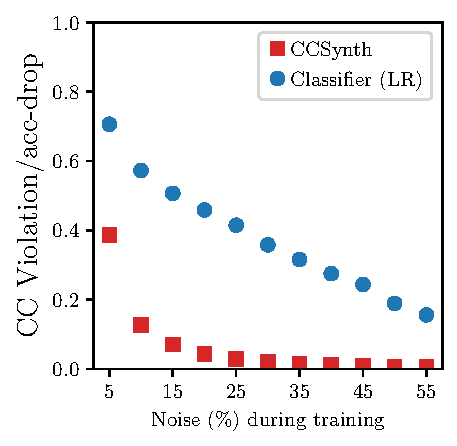
\includegraphics[width=\linewidth]{Plots/Figure_6_b.pdf}
	\vspace{-5mm}
	\caption{}
	\label{fig:har-ml-experiment-noise}
	\end{subfigure}	
	\begin{subfigure}[t]{0.16\textwidth}
		\centering
		\includegraphics[width=\linewidth]{Plots/Figure_6_c.pdf}
	\vspace{-5mm}
	\caption{}
	\label{fig:gradual-drift-har}
	\end{subfigure}
	\vspace{-5mm}	
	\caption{(a)~As a higher fraction of mobile activity data is mixed with
sedentary activity data, \dis are violated more, and the classifier's
mean accuracy-drop increases. 
%
(b)~\revisetwo{As more noise is added during training, \dis get weaker,
leading to less violation and decreased accuracy-drop.}
%
(c)~\system detects the gradual local drift on the
HAR dataset as more people start changing their
activities. In contrast, weighted-PCA (W-PCA) fails to detect drift in absence of
a strong global drift.} 
		\vspace{2mm}	
	\centering
	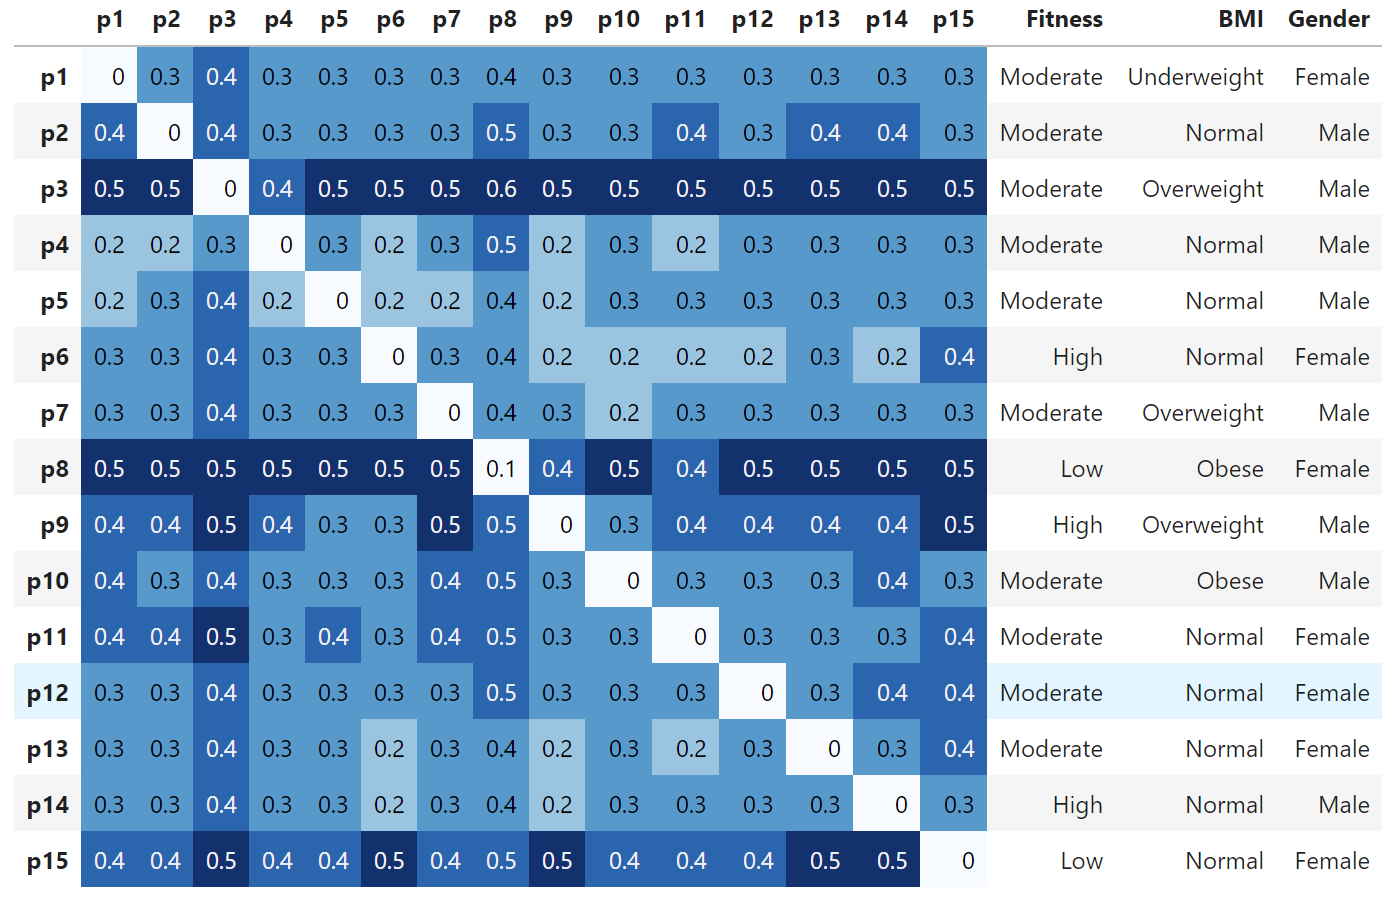
\includegraphics[width=1\linewidth]{Figures/Figure_7.png}
		\vspace{-7mm}	
	\caption{\looseness-1 Inter-person \invariant violation heat map. Each person has a very low self-violation.}
	\label{fig:har-inter-person-drift-heatmap}
		\vspace{1mm}	
	\centering
\end{figure}

\smallskip

\subsection{Data Drift}\label{exp-invariants-for-drift}
%
% \looseness-1
We now present results of using \dis for drift-detection; specifically, for
\emph{quantifying} drift in data. Given a baseline dataset $D$, and a new
dataset $D'$, we measure the drift as average violation of tuples in $D'$ on
\dis learned for $D$.

\smallskip

\noindent\textbf{HAR.} We perform two drift-quantification experiments on
HAR:

\smallskip

\noindent \emph{Gradual drift.} \looseness-1 For observing how \system detects
gradual drift, we introduce drift in an organic way. The initial training
dataset contains data of exactly one activity for each person. This is a
realistic scenario as one can think of it as taking a snapshot of what a group
of people are doing during a reasonably small time window. We introduce gradual
drift to the initial dataset by altering the activity of one person at a time.
To control the amount of drift, we use a parameter $K$. \reviseone{When $K =
1$, the first person switches their activity, i.e., we replace the tuples
corresponding to the first person performing activity A with new tuples that
correspond to the same person performing another activity B.} When $K = 2$, the
second person switches their activity in a similar fashion, and so on. As we
increase $K$ from $1$ to $15$, we expect a gradual increase in the drift
magnitude compared to the initial training data. When $K = 15$, all persons
have switched their activities from the initial setting, and we expect to
observe maximum drift. We repeat this experiment $10$ times, and display the
average \invariant violation in Fig.~\ref{fig:gradual-drift-har}: the drift
magnitude (violation) indeed increases as more people alter their activities.

\begin{figure*}[t]
	\centering	
	\includegraphics[width=.8\linewidth]{Plots/Figure_8.pdf}	
		\vspace{-5mm}
	 \caption{In the EVL benchmark, \system quantifies drift correctly for all
	 cases, outperforming other approaches. PCA-SPLL fails to detect drift in a few cases by
 	 discarding all principal components; CD-MKL and CD-Area are too sensitive to
 	 small drift and detect spurious drifts.}
	\vspace{-2mm}
	\label{fig:drift-baseline-comparison-EVL}
\end{figure*}

The baseline weighted-PCA approach (W-PCA) fails to model local \invariants
(who is doing what), and learns some weaker global \invariants indicating that
``a group of people are performing some activities''. Thus, it fails to detect
the gradual local drift. \system can detect drift when individuals switch
activities, as it learns \emph{disjunctive} \invariants that encode who is
doing what.

\smallskip


\noindent \looseness-1 \emph{Inter-person drift.} \reviseone{The goal of this
experiment is to observe how effectively \dis can model the representation of an
entity and whether such learned representations can be used to accurately
quantify drift between two entities.} We use half of each person's data to
learn the \invariants, and compute violation on the held-out data. \system
learns disjunctive \invariants for each person over all activities, and then we
use the violation w.r.t.\ the learned \invariants to measure how much the other
persons drift. While computing drift between two persons, we compute
activity-wise \invariant violation scores and then average them out. In
Fig.~\ref{fig:har-inter-person-drift-heatmap}, the violation score at row
\texttt{p1} and column \texttt{p2} denotes how much \texttt{p2} drifts from
\texttt{p1}. As one would expect, we observe a very low self-drift across the
diagonal. Interestingly, our result also shows that some people are more
different from others, which appears to have some correlation with (the hidden
ground truth) fitness and BMI values. This asserts that the \invariants we
learn for each person are an accurate abstraction of that person's activities,
as people do not deviate too much from their usual activity patterns.




\smallskip

\noindent \textbf{EVL.} We now compare \system against other state-of-the-art
drift detection approaches on the EVL benchmark.

\smallskip

\noindent\emph{Baselines.}
%
We use two drift-detection baselines as described below:

\smallskip

(1)~PCA-SPLL~\cite{DBLP:journals/tnn/KunchevaF14} 
%\footnote{\scriptsize{SPLL
%source code: }\scriptsize{\url{github.com/LucyKuncheva/Change-detection}}},
similar to us, also argues that principal components with lower variance are
more sensitive to a general drift, and uses those for dimensionality reduction.
It then models multivariate distribution over the reduced dimensions and
applies semi-parametric log-likelihood (SPLL) to detect drift between two
multivariate distributions. However, PCA-SPLL discards all high-variance
principal components and does not model disjunctive \invariants.

\smallskip
 
(2)~CD (Change Detection)~\cite{DBLP:conf/kdd/QahtanAWZ15}
%\footnote{\scriptsize{CD source code:}
%\scriptsize{\url{mine.kaust.edu.sa/Pages/Software.aspx}}} 
is another PCA-based approach for drift detection in data streams. But unlike
PCA-SPLL, it ignores low-variance principal components. CD projects the data
onto top $k$ high-variance principal components, which results into multiple
univariate distributions. We compare against two variants of CD: CD-Area, which
uses the intersection area under the curves of two density functions as a
divergence metric, and CD-MKL, which uses Maximum KL-divergence as a symmetric
divergence metric, to compute divergence between the univariate distributions.

\smallskip

\looseness-1 Fig.~\ref{fig:drift-baseline-comparison-EVL} depicts how \system
compares against CD-MKL, CD-Area, and PCA-SPLL, on 16 datasets in the
EVL benchmark. For PCA-SPLL, we retain principal components that contribute to
a cumulative explained variance below 25\%. Beyond drift detection, which just
detects if drift is above some threshold, we focus on drift
quantification. A tuple $(x,y)$ in the plots denotes that drift
magnitude for dataset at $x^{th}$ time window, w.r.t.\ the dataset at the first
time window, is $y$. Since different approaches report drift magnitudes in
different scales, we normalize the drift values within $[0, 1]$. Additionally,
since different datasets have different number of time windows,
for the ease of exposition, we normalize the time window indices. Below
we state our key findings from this experiment:
% in a similar way (determined by the data and
%window sizes). 

%  $\mathbf{c} = \{ c_0, \ldots, c_n\}$ within the
% range [0, 1] by using a simple transformation: $ \hat{c_i} = \frac{c_i -
% \min(\mathbf{c})} {\max(\mathbf{c}) - \min(\mathbf{c})}$.

\smallskip 

 
\looseness-1 \emph{\system's drift quantification matches the ground truth.} In
all of the datasets in the EVL benchmark, \system is able to correctly quantify
the drift, which matches the ground truth~\cite{evlVideo} exceptionally well.
In contrast, as CD focuses on detecting the drift point, it is ill-equipped to
precisely quantify the drift, which is demonstrated in several cases (e.g.,
2CHT), where CD fails to distinguish the deviation in drift magnitudes. In
contrast, both PCA-SPLL and \system correctly quantify the drift.
\revisetwo{Since CD only retains high-variance principal components, it is more
susceptible to noise and considers noise in the dataset as significant drift,
which leads to incorrect drift quantification. In contrast, PCA-SPLL and
\system ignore the noise and only capture the general notion of drift.}
% In all
% of the EVL datasets, we found CD-Area to work better than CD-MKL, which also
% agrees with the authors' experiments.


\smallskip

\looseness-1 \emph{\system models local drift.} When the dataset contains
instances from multiple classes, the drift may be just local, and not global
(e.g., 4CR dataset~\citeTechRep). In such cases, PCA-SPLL fails to detect drift
(4CR, 4CRE-V2, and FG-2C-2D). In contrast, \system learns disjunctive
\invariants and quantifies local drifts accurately.


\smallskip
\noindent
\fbox{
\parbox{0.95\columnwidth}{
\emph{Key takeaways:} 
%
\system can effectively detect data drift, both global and local, is robust
across drift patterns, and significantly outperforms the state-of-the-art
methods.}
%
}

\ignore{
\subsection{Explaining Non-conformance}\label{sec:extune}

When a serving dataset is determined to be sufficiently different or drifted
from the training set, the next step often is to characterize the difference. A
common way of characterizing these differences is to perform a causality or
responsibility analysis to determine which attributes are most responsible for
the observed drift (non-conformance). We use the violation values produced by
\dis, along with well-established principles of causality, to quantify
responsibility for non-conformance.

\smallskip 

\noindent\textbf{\extune.} \looseness-1 We built a tool
\extune~\cite{DBLP:conf/sigmod/FarihaTRG20}\footnote{Anonymized due to double
blind consideration.}, on top of \system, to compute the
responsibility values as described next. Given a training dataset $D$ and a
non-conforming tuple $t \in {\DDom}^m$, we measure the \emph{responsibility} of
the $i^{th}$ attribute $A_i$ towards the non-conformance as follows: (1)~We
intervene on $t.A_i$ by altering its value to the mean of $A_i$ over $D$ to
obtain the tuple $t^{(i)}$. (2)~In $t^{(i)}$, we compute how many additional
attributes need to be altered to obtain a tuple with no violation. If $K$
additional attributes need to be altered, $A_i$ has responsibility
$\frac{1}{K+1}$. (3)~This responsibility value for each tuple $t$ can be
averaged over the entire serving dataset to obtain an aggregate responsibility
value for $A_i$.
%
Intuitively, for each tuple, we are ``fixing'' the value of $A_i$ with a
``more typical'' value, and checking how close (in terms of additional fixes required) this takes us to a conforming tuple.
The larger the number of additional fixes required, the lower the responsibility of $A_i$.


\begin{figure}
	\centering
	%
	\begin{subfigure}{.09\textwidth}
	  \centering
	  \includegraphics[width=\linewidth, height=40mm]{Figures/cardio.pdf}
	  \caption{}
	  \label{cardio}
	\end{subfigure}
	\hspace{-1mm}
	\begin{subfigure}{.09\textwidth}
	  \centering
	  \includegraphics[width=\linewidth, height=40mm]{Figures/mobileprice.pdf}
	  \caption{}
	  \label{mobilePrice}
	\end{subfigure}
	\hspace{-1.5mm}
	\begin{subfigure}{.09\textwidth}
	  \centering
	  \includegraphics[width=\linewidth, height=40mm]{Figures/houseprice.pdf}
	  \caption{}
	  \label{housePrice}
	\end{subfigure}
	\hspace{-1.5mm}
	\begin{subfigure}{.2\textwidth}
		\centering
		\includegraphics[width=.9\linewidth, height=40mm]{Figures/LED-drift.pdf}
	  	\caption{}
	    \label{fig:LED-drift}
	\end{subfigure}
	\vspace{-3mm}
	%
	\caption{Responsibility assignment on attributes for drift on 
	(a)~Cardiovascular disease: trained on patients with no disease and served on patients with disease,
	(b)~Mobile Prices: trained on cheap mobiles and served on expensive mobiles and 
	(c)~House Prices: trained on house with price $<=$ 100K and served on house with price $>=$ 300K.
	(d)~Detection of drift on LED dataset. The dataset drifts every 5
		 windows (25,000 tuples). At each drift, a certain set of LEDs
		 malfunction and take responsibility of the drift.}
	\label{fig:extune}
	\vspace{-7mm}
\end{figure}

\begin{figure}
	\centering


\end{figure}

% Does the word intervenes have a special meaning? Do we need to retain it? 
\smallskip

\noindent\textbf{Case studies.} \extune produces bar-charts of responsibility
values as depicted in Fig.~\ref{fig:extune}.
Figures~\ref{cardio},~\ref{mobilePrice}, and~\ref{housePrice} show the
explanation results for Cardiovascular Disease, Mobile Price, and House Price
datasets, respectively. For the cardiovascular disease dataset, the training
and serving sets consist of data for patients without and with cardiovascular
disease, respectively. For the House Price and Mobile Price datasets, the
training and serving sets consist of houses and mobiles with prices below and
above a certain threshold, respectively. As one can guess, we get many useful
insights from the non-conformance responsibility bar-charts such as: ``abnormal
(high or low) blood pressure is a key cause for non-conformance of patients
with cardiovascular disease w.r.t. normal people'', ``RAM is a distinguishing
factor between expensive and cheap mobiles'', ``the reason for houses being
expensive depends holistically on several attributes''.

Fig.~\ref{fig:LED-drift} shows a similar result on the LED dataset. Instead
of one serving set, we had 20 serving sets (the first set is also used as a training
set to learn \dis). We call each serving set a window where each window
contains 5,000 tuples. This dataset introduces gradual concept drift every
25,000 rows (5 windows) by making a subset of LEDs malfunctioning. As one can
clearly see, during the initial 5 windows, no drift is observed. In the next 5
windows, LED 4 and LED 5 starts malfunctioning; in the next 5 windows, LED 1
and LED 3 starts malfunctioning, and so on.
}

\section{Related Work}\label{sec:applications}
%!TEX root = paper.tex

There is extensive literature on
data-profiling~\cite{DBLP:journals/vldb/AbedjanGN15} primitives that model
relationships among data attributes, such as functional dependencies
(FD)~\cite{papenbrock2015functional, DBLP:conf/sigmod/ZhangGR20} and their
variants~\cite{koudas2009metric, DBLP:conf/icde/FanGLX09,
DBLP:conf/sigmod/IlyasMHBA04, huhtala1999tane, kruse2018efficient,
caruccio2016discovery, qahtan2020pattern}, differential
dependencies~\cite{song2011differential}, denial
constraints~\cite{DBLP:journals/pvldb/ChuIP13,
DBLP:journals/corr/abs-2005-08540, DBLP:journals/pvldb/BleifussKN17,
pena2019discovery}, statistical constraints~\cite{DBLP:conf/sigmod/YanSZWC20},
etc. However, none of them focus on learning approximate arithmetic
relationships that involve multiple numerical attributes in a noisy setting,
which is the focus of our work. Some FD
variants~\cite{DBLP:conf/sigmod/IlyasMHBA04, koudas2009metric, huhtala1999tane,
kruse2018efficient, caruccio2016discovery} consider noisy setting, but they
require noise parameters to be explicitly specified by the user. In contrast,
we do not require any explicit noise parameter.


The issue of trust, resilience, and interpretability of artificial intelligence
(AI) systems has been a theme of increasing interest
recently~\cite{DBLP:conf/cav/Jha19, DBLP:journals/crossroads/Varshney19,
DBLP:journals/corr/abs-1904-07204, DBLP:conf/mlsys/KangRBZ20}, particularly for
safety-critical data-driven AI systems~\cite{DBLP:journals/bigdata/VarshneyA17,
DBLP:conf/hicons/TiwariDJCLRSS14}. A standard way to decide whether to trust a
classifier or not, is to use the classifier-produced confidence score. However,
this is not always effective since the classifier's confidence scores are not
well-calibrated~\cite{DBLP:conf/nips/JiangKGG18}. While some recent
techniques~\cite{DBLP:conf/nips/JiangKGG18, DBLP:conf/sigmod/SchelterRB20,
DBLP:journals/corr/HendrycksG16c, DBLP:journals/corr/abs-1812-02765} aim at
validating the inferences made by machine-learned models on unseen tuples, they
usually require knowledge of the inference task, access to the model, and/or
expected cases of data shift, which we do not. Furthermore, they usually
require costly hyper-parameter tuning and do not generate closed-form data
profiles like \dis (Fig.~\ref{relatedWorkMatrix}). Prior work on data drift,
change detection, and covariate shift~\cite{DBLP:conf/sigmod/Aggarwal03,
DBLP:journals/tnn/BuAZ18, dasu2006information, DBLP:journals/eswa/MelloVFB19,
DBLP:conf/kdd/ReisFMB16, DBLP:journals/inffus/FaithfullDK19,
DBLP:conf/icml/Ho05, hooi2019branch, DBLP:conf/sdm/KawaharaS09,
DBLP:conf/vldb/KiferBG04, DBLP:journals/eswa/SethiK17, DBLP:conf/kdd/SongWJR07,
DBLP:conf/sac/IencoBPP14, DBLP:conf/cbms/TsymbalPCP06,
DBLP:journals/corr/WangA15, DBLP:conf/sbia/GamaMCR04, DBLP:conf/sdm/BifetG07,
gaber2006classification, DBLP:journals/tnn/RutkowskiJPD15,
DBLP:conf/iri/SethiKA16} relies on modeling data distribution. However, data
distribution does not capture constraints, which is the primary focus of our
work.


Few works~\cite{DBLP:journals/corr/abs-1812-02765,
DBLP:journals/corr/HendrycksG16c, DBLP:journals/corr/abs-1909-03835} use
autoencoder's~\cite{hinton2006reducing, rumelhart1985learning} input
reconstruction error to determine if a new data point is out-of-distribution.
Our approach is similar to outlier-detection~\cite{kriegel2012outlier} and
one-class-classification~\cite{DBLP:conf/icann/TaxM03}. However, \dis differ
from these approaches as they perform under the additional requirement to
generalize the data in a way that is exploited by a given class of ML models.
In general, there is a clear gap between representation learning (that models
data likelihood)~\cite{hinton2006reducing, rumelhart1985learning,
achlioptas2017learning, karaletsos2015bayesian} and the (constraint-oriented)
data-profiling techniques to address the problem of trusted AI and our aim is
to bridge this gap.

\vspace{-1mm}











\section{Summary and Future Directions}\label{discussion}
%!TEX root = paper.tex
%\section{Summary and Future Directions}
\looseness-1
We introduced \dis, and the notion of \nc tuples for trusted
machine learning. We presented an efficient and scalable approach for
synthesizing \dis and empirically demonstrated their effectiveness in tagging
\nc tuples and quantify data drift.
% The experiments validate our theory and our principle of using low-variance
% \views to generate effective \dis.
We studied two use-cases from a large pool of potential applications using
linear \dis. In future, we want to explore more powerful nonlinear \dis using
autoencoders. Moreover, we plan to explore approaches to learn \dis in a
decision-tree-like structure where categorical attributes will guide the
splitting conditions and leaves will contain simple \dis.





\smallskip

{\noindent \textbf{Acknowledgements}: This work was partially
supported by the NSF grants IIS-1453543 and CCF-1763423, and by Oracle Labs.}
%, and a Microsoft Research Dissertation Grant.}

\balance
\bibliographystyle{ACM-Reference-Format}
\bibliography{paper}

\ifTechRep
\appendix
\input{9_appendix}
\fi 

\end{document}
